\documentclass{article}
\usepackage[spanish]{babel}
\usepackage[utf8]{inputenc}
\usepackage[letterpaper,top=2cm,bottom=2cm,left=3cm,right=3cm,marginparwidth=1.75cm]{geometry}
\usepackage{amsmath}
\usepackage[colorlinks=true, allcolors=blue]{hyperref}
\usepackage{makeidx}
\usepackage{fancyhdr}
\usepackage{xcolor}
\usepackage[document]{ragged2e}
\usepackage{imakeidx}
\usepackage{hyperref}
\usepackage{graphicx}
\usepackage{wrapfig}
\usepackage{xcolor}
\usepackage{tabularx}
\usepackage{graphicx}
\definecolor{rojo}{RGB}{255,0,0}
\definecolor{azul}{RGB}{12,0,200}

%Configurar el encabezado de pagina
\pagestyle{fancy}
\lhead{Análisis y Diseño de Sistemas}
\chead{}
\rhead{5CM4 - Análisis y Diseño de Sistemas}
\renewcommand{\headrulewidth}{0.4pt} % Ancho de la línea horizontal del encabezado

% Cargar el paquete makeidx para el índice
\makeindex

%\begin{document}
%Portada
\begin{document}
\begin{titlepage}
\centering
{\bfseries\LARGE Instituto Politécnico Nacional \par}
\vspace{.5cm}
{\bfseries\LARGE Escuela Superior de Computo \par}
\vspace{1cm}
\Large ANÁLISIS Y DISEÑO DE SISTEMAS \par
\vspace{1cm}
\itshape\LARGE Proyecto \par
\vspace{1cm}
%\itshape\LARGE Requerimientos funcionales, no funcionales y reglas de negocio \par
%\vspace{2cm}
\LARGE 5CM4\par
\vspace{1cm}

\begin{FlushLeft}
\Large Nombre del equipo: Bellakitos FC\par
\Large Nombre del proyecto: \textbf{Beyamaps}\par
\vspace{0.5cm}
\Large Profesora: Maldonado Castillo Idalia	 \par
\vspace{0.5cm}
    Integrantes:\\
    \begin{enumerate}
    \item Alvarado Díaz Dario\\
   \item Cervantes Maxtla Saúl\\
    \item Dominguez Olvera Leonardo Daniel\\
    \item Espinosa de los Monteros Martínez Eric Omar\\
   \item Estrada Yepez Omar Said\\
   \item García Torres Adair\\
   \item Ledesma Ramírez José Emiliano\\
   \item Murillo Mendoza María Fernanda\\
   \item Peña Ramírez Jonathan\\
   \item Ramírez Martínez Kevin Andrés\\
   \item Rojo Segura José Emmanuel\\
   \item Zamarrón Ramírez Javier\\
    \end{enumerate}
\vspace{.5cm}
\Large Fecha de Entrega: 18 de Octubre de 2023 \par
\vspace{.5cm}
\end{FlushLeft}
\end{titlepage}
\tableofcontents
\newpage
\section{Alcance del proyecto}
\justifying
Sistema que fomente el turismo el cual sera una aplicación movil, donde el turista que lo use se le mostrara en un mapa su ubicacion geografica a traves de su GPS y sea capaz de recomendarle sitios turisticos cercanos a su ubicacion para visitar de acuerdo a su medio de transporte ya sea caminando o utilizando un vehiculo. Los sitios turisticos deberan tener una clasificación como museos, restaurantes, parques entre otros sitios de interes. El sistema solo sera funcional a nivel nacional, es decir, solamente en México.

\section{Requerimientos Funcionales}
\subsection{Usuario Turista}
\begin{itemize}
    \item El sistema deberá acceder a la ubicación del usuario turista por medio de su GPS.
    \item El sistema debe permitir al usuario turista buscar lugares cercanos en el mapa basados en su ubicación en un radio de 1 km a 10 km.
    \item El sistema debe permitir al usuario turista la creación de un perfil mediante un correo y una contraseña.
    \item El sistema debe permitir al usuario turista iniciar sesión.
    \item El sistema debe permitir al usuario turista cerrar sesión.
    \item El sistema debe permitir al usuario turista visualizar sus datos tales como nombre, correo electronico. 
    \item El sistema debe permitir al usuario turista modificar sus datos tales como nombre, correo, preferencias, radio de búsqueda y contraseña.
    \item El sistema deberá mostrar al usuario turista las reseñas de cada sitio de interés.
    \item El sistema permitirá al usuario turista crear itinerarios con base a los sitios de interes, en un dia determinado y poder seleccionar una hora de inicio para cada sitio.
    \item El sistema permitira la eliminación de los lugares de su itinerario o todo el itinerario.
    \item El sistema deberá permitir al perfil usuario turista guardar ubicaciones en favoritos y poder eliminarlos.
    \item El sistema deberá generar una ruta basada en los lugares listados en el itinerario partiendo de la ubicación del usuario turista.
    \item El sistema deberá permitir al usuario turista seleccionar su forma de movilidad.
    \item El sistema deberá permitir al usuario turista eliminar su cuenta.
    \item El sistema deberá mostrar información de los lugares señalados tales como su nombre, dirección, horarios, calificación, distancia y opciones de agregar itinerario, visitado y agregar a favoritos.
    \item El sistema debe permitir al usuario turista recuperar su contraseña utilizando su correo electronico.
    \item El sistema debera mostrar los sitios visitados y la posibilidad de eliminarlos.
    \item El sistema permitira realizar la busqueda de sitios de interes.
    \item El sistema debera mostrar el sitio de interes en el mapa.
\end{itemize}

\subsection{Usuario Administrador}
\begin{itemize}
    \item El sistema deberá permitir al usuario administrador visualizar y actualizar los datos del usuario turista.
    \item El sistema deberá permitir al usuario administrador suspender y/o eliminar cuentas del usuario turista.
   \item El sistema deberá permitir al usuario administrador iniciar y cerrar sesión.
 \end{itemize}

\section{Requerimientos No Funcionales}
\begin{enumerate}
    \item Los datos de ubicación del usuario turista deberán ser utilizados por el sistemas mientras este ultimo se encuentre en funcionamiento.
    
    \item El sistema debe solicitar al usuario turista permiso para utilizar su ubicación a través de una ventana emergente al momento de iniciaizar el sistema por primera vez.
    
    \item El sistema deberá dar acceso a los usuarios turista en un tiempo aproximado de 3 minutos como maximo.

\item El sistema debe permitir al usuario visualizar sus datos, al hacer clic en "mi perfil". La sección de datos
de la cuenta debe mostrar al usuario información detallada sobre su perfil.

\item El sistema debe permitir al usuario turista la modificación de sus datos, preferencias y eliminar cuenta por medio de una validación de su contraseña. 

\item El sistema permitira al ususario turista agregar los lugares mediante un boton \textbf{Agregar itinerario} que se muestra en el apartado detalles del lugar a la sección itinerario

\item El sistema permitira elegir en que horarios llegara el usuario turista a cada uno de los lugares mostrados en la sección itinerario. El sistema ordenara el itinerario con base a las horas idicadas de menor a mayor. El usuario debe poder modificar los horarios de los lugares a visitar cuando lo desee.

\item El sistema permitira al usuario turista marcar como visitado el lugar en la sección itinerario, agruegando el lugar al historial.

\item  El sistema debera validar la eliminacion de los lugares del itinerario, historial, favoritos a traves de una confirmación del usuario turista mostrada en una ventana emergente.

\item El sistema debera generar una ruta a partir de un itinerario, la generacion de la ruta se dara de acuerdo a la movilidad seleccionada por el usuario turista ya sea a pie, auto o transporte publico. La ruta generada se mostrara en una nueva pantalla que aparecera el mapa y los lugares indicados con su ubicacion y el orden que debera seguir.

\item El sistema debera permitir mostrar los lugares en el mapa. El usuario debe poder dar click a los diferentes lugares, el sistema debera mostrar informacion del lugar y un boton que indique ver detalles del lugar seleccionado.

\item El sistema debera mostrar la informacion del lugar indicado. El usuario turista debe poder seleccionar agregar a itinerario, marcar como visitado y/o como favorito. De acuerdo a su elección se agregara a su apartado correspondiente.

\item El usuario debe poder buscar diferentes lugares en los buscadores las secciones pantalla mapa, itinerario, historial y favoritos. EL sistema debera mostrar los lugares relacionados a la palabra colocada, Se debera ver la visualizacion de su nombre e imagen del lugar.

\item El sistema permitira la visualizacion de los lugares favoritos del usuario turista. El usuario debe poder agregar y/o eliminar sus favoritos. El sistema debera permitir buscar sus lugares favoritos mediante la opcion de busqueda.

\item El sistema permitira la visualizacion de su historial del usuario turista en una nueva pantalla. El usuario turista debe poder seleccionar ver detalles y eliminar historial completo. El usuario puede buscar sus lugares visitado mediante la opcion de busqueda. El sistema debe poder eliminar el historial.
    
    \item Los datos de los usuarios turista, como su informacion personal, correo y contraseña seran protegidos mediante un cifrado.
    
    \item El sistema debe implementar mecanismos de autenticación para proteger los datos de los usuarios turistas y garantizar que solo tengan acceso a su propia información, atraves de su nombre de usuario y correo electronico.

    \item El sistema debera verificar en la base de datos los correos electronicos, con la finalidad de que sean unicos para los usuarios turistas al momento del registro de una nueva cuenta. Los correos electronicos solo pueden ser utilizados una unica vez en una cuenta.

    \item El sistema deberá ser responsivo en dispositivos móviles con pantallas a partir de una resolución de 375x667 px hasta 820x1180.
    
    \item El sistema deberá ser responsivo en dispositivos de cómputo con pantallas de una resolución de 1280x720 px.
    
    \item El sistema debe ser capaz de integrarse con servicios de mapas y navegación para proporcionar direcciones y rutas precisas a partir de la API de Google.
    
    \item El sistema debe ser capaz de manejar al menos 20 usuarios concurrentes sin degradación significativa del rendimiento utilizando balanceadores de carga.
    
    \item La precisión de la ubicación debe ser lo más precisa posible, al menos 2 km, teniendo en cuenta las capacidades del hardware del dispositivo del usuario turista a través de la activación del GPS de dicho dispositivo.
    
    \item El sistema no deberá estar disponible únicamente en periodos de mantenimiento previamente señalados al usuario turista a traves de notificaciones por medio del sistema.
    
    \item El sistema deberá cerrar la sesión del usuario turista cuando él lo indique, la sesión cerrara de manera inmediata y redirigir al usuario turista a la página de inicio de sesión y debera recibir un mensaje de confirmación que indique que la sesión se ha cerrado de manera exitosa y segura. 
    
    \item El sistema debe contar con medidas de seguridad para evitar un usuario pueda acceder a la cuenta de otro usuario mientras este abierta su sesión en un dispositivo que ha dejado su sesión abierta, por lo tanto solo se tendria una sesion iniciada en un unico dispositivo.
    

\item  El sistema permitira al usuario turista la recuperación de su contraseña en el apartado de iniciar sesion, mediante su correo electronico registrado previamente al momento de la creacion de su cuenta validando la información proporcionada a traves de un enlace. La contraseña sera actualizada teniendo que confirmar la nueva contraseña para su actualización.
\end{enumerate}

\section{Reglas de Negocio}
\begin{enumerate}
    \item \textbf{Registro de Usuarios}:
    \begin{itemize}
        \item El sistema no deberá permitir el registro de dos usuarios con la misma dirección de correo electrónico ni con el mismo nombre de usuario.
        \item Los usuarios turistas pueden crear un perfil proporcionando un correo electrónico de gmail y contraseña válidos, así como sus datos personales como nombre, teléfono, y preferencias de lugares de interés.
        \item Las contraseñas deberán tener al menos una letra mayúscula y un carácter especial (*,@, -), tener una longitud mínima de 8 caracteres y máxima de 12 y utilizar caracteres alfanuméricos.
        \item El nombre de usuario sera unico para cuenta, solamente existira uno en el sistema con esos datos, sin tener espacios y debera ser de una longitud minima de 10 caracteres y maxima 15 caracteres.
        \item La contraseña deberan ser escritas 2 veces, una para ingreso y otra para validación, ambas deben contener los mismos caracteres para su confirmación.
        \item Los nombres y apellidos deberan ser caracteres alfabeticos de una longitud maxima de 60 caracteres. para cada uno.
        \item El correo electrónico debera ser de GMAIL.
        \item El telefono movil debe ser de 10 caracteres numericos.
        
    \end{itemize}

    
    \item \textbf{Inicio de Sesión}:
    \begin{itemize}
        \item Los usuarios turistas deben iniciar sesión con su correo electrónico y contraseña registrados.
        \item El sistema debe verificar las credenciales del usuario antes de permitir el acceso.
    \end{itemize}
    
    \item \textbf{Acceso a la Ubicación}:
    \begin{itemize}
        \item El sistema debe obtener el consentimiento del usuario turista para acceder a su ubicación por medio de una ventana emergente cuando se abra por primera el sistema.
        \item El acceso a la ubicación debe ser desactivable por parte del usuario en cualquier momento.
    \end{itemize}
    
    \item \textbf{Búsqueda de Lugares Cercanos}:
    \begin{itemize}
        \item El usuario turista podrá filtrar la búsqueda seleccionando las categorías de su preferencia tales como restaurantes, parques, museos, entre otros.
        \item Los usuarios turistas pueden buscar lugares de interés dentro de un radio de 1 km a 10 km de su ubicación actual.
        \item Los resultados de la búsqueda deben basarse en la ubicación actual del usuario.
    \end{itemize}
    

    
    \item \textbf{Visualización/Modificación de Datos de Perfil}:
    \begin{itemize}
        \item Los usuarios turistas pueden ver y editar su nombre, región, sitios de interés, radio de búsqueda, contraseña.
        \item Los usuarios turistas solo visualizarán los datos de nombre de usuario y correo electrónico sin realizar modificaciones.
    \end{itemize}

    \item \textbf{Creación de Itinerarios}:
    \begin{itemize}
        \item Los usuarios turistas pueden crear itinerarios basados en la cercanía y horarios de los lugares de interés.
        \item Deben especificar la fecha y hora de inicio de cada itinerario.
        \item Solo se tendra un itinerario por dia indicado.
    \end{itemize}
    
    \item \textbf{Guardado de Ubicaciones en Favoritos}:
    \begin{itemize}
        \item Los usuarios turistas pueden guardar lugares de interés en su lista de favoritos para acceder fácilmente en el futuro.
    \end{itemize}
    
    \item \textbf{Selección de Forma de Desplazamiento}:
    \begin{itemize}
        \item Los usuarios turistas pueden elegir su forma de desplazamiento preferida, como caminar, conducir, o usar transporte público (PENDIENTE).
    \end{itemize}
    
    \item \textbf{Privacidad de Datos}:
    \begin{itemize}
        \item Los usuarios turistas deberán aceptar los términos y condiciones mostrados al momento de crear una cuenta.
        \item Los datos personales de los usuarios, como el correo electrónico y la ubicación, deben mantenerse confidenciales y protegerse de acuerdo con las regulaciones de privacidad aplicables (CUALES).
    \end{itemize}
    
    \item \textbf{Borrado de Cuentas}:
    \begin{itemize}
        \item Los usuarios turistas pueden eliminar sus cuentas de usuario si lo desean, lo que resultará en la eliminación permanente de sus datos.
    \end{itemize}
    \item \textbf{Verificación de cuentas}:
    \begin{itemize}
        \item El sistema generara un token para los procesos de restablecer contraseña, el cual tendra una duración de 30 min activo.
    \end{itemize}
\end{enumerate}

%ARCHIVO DE DIAGRAMAS
\section{Diagrama de Casos de Uso}
    \begin{figure}[htbp]
        \centering
        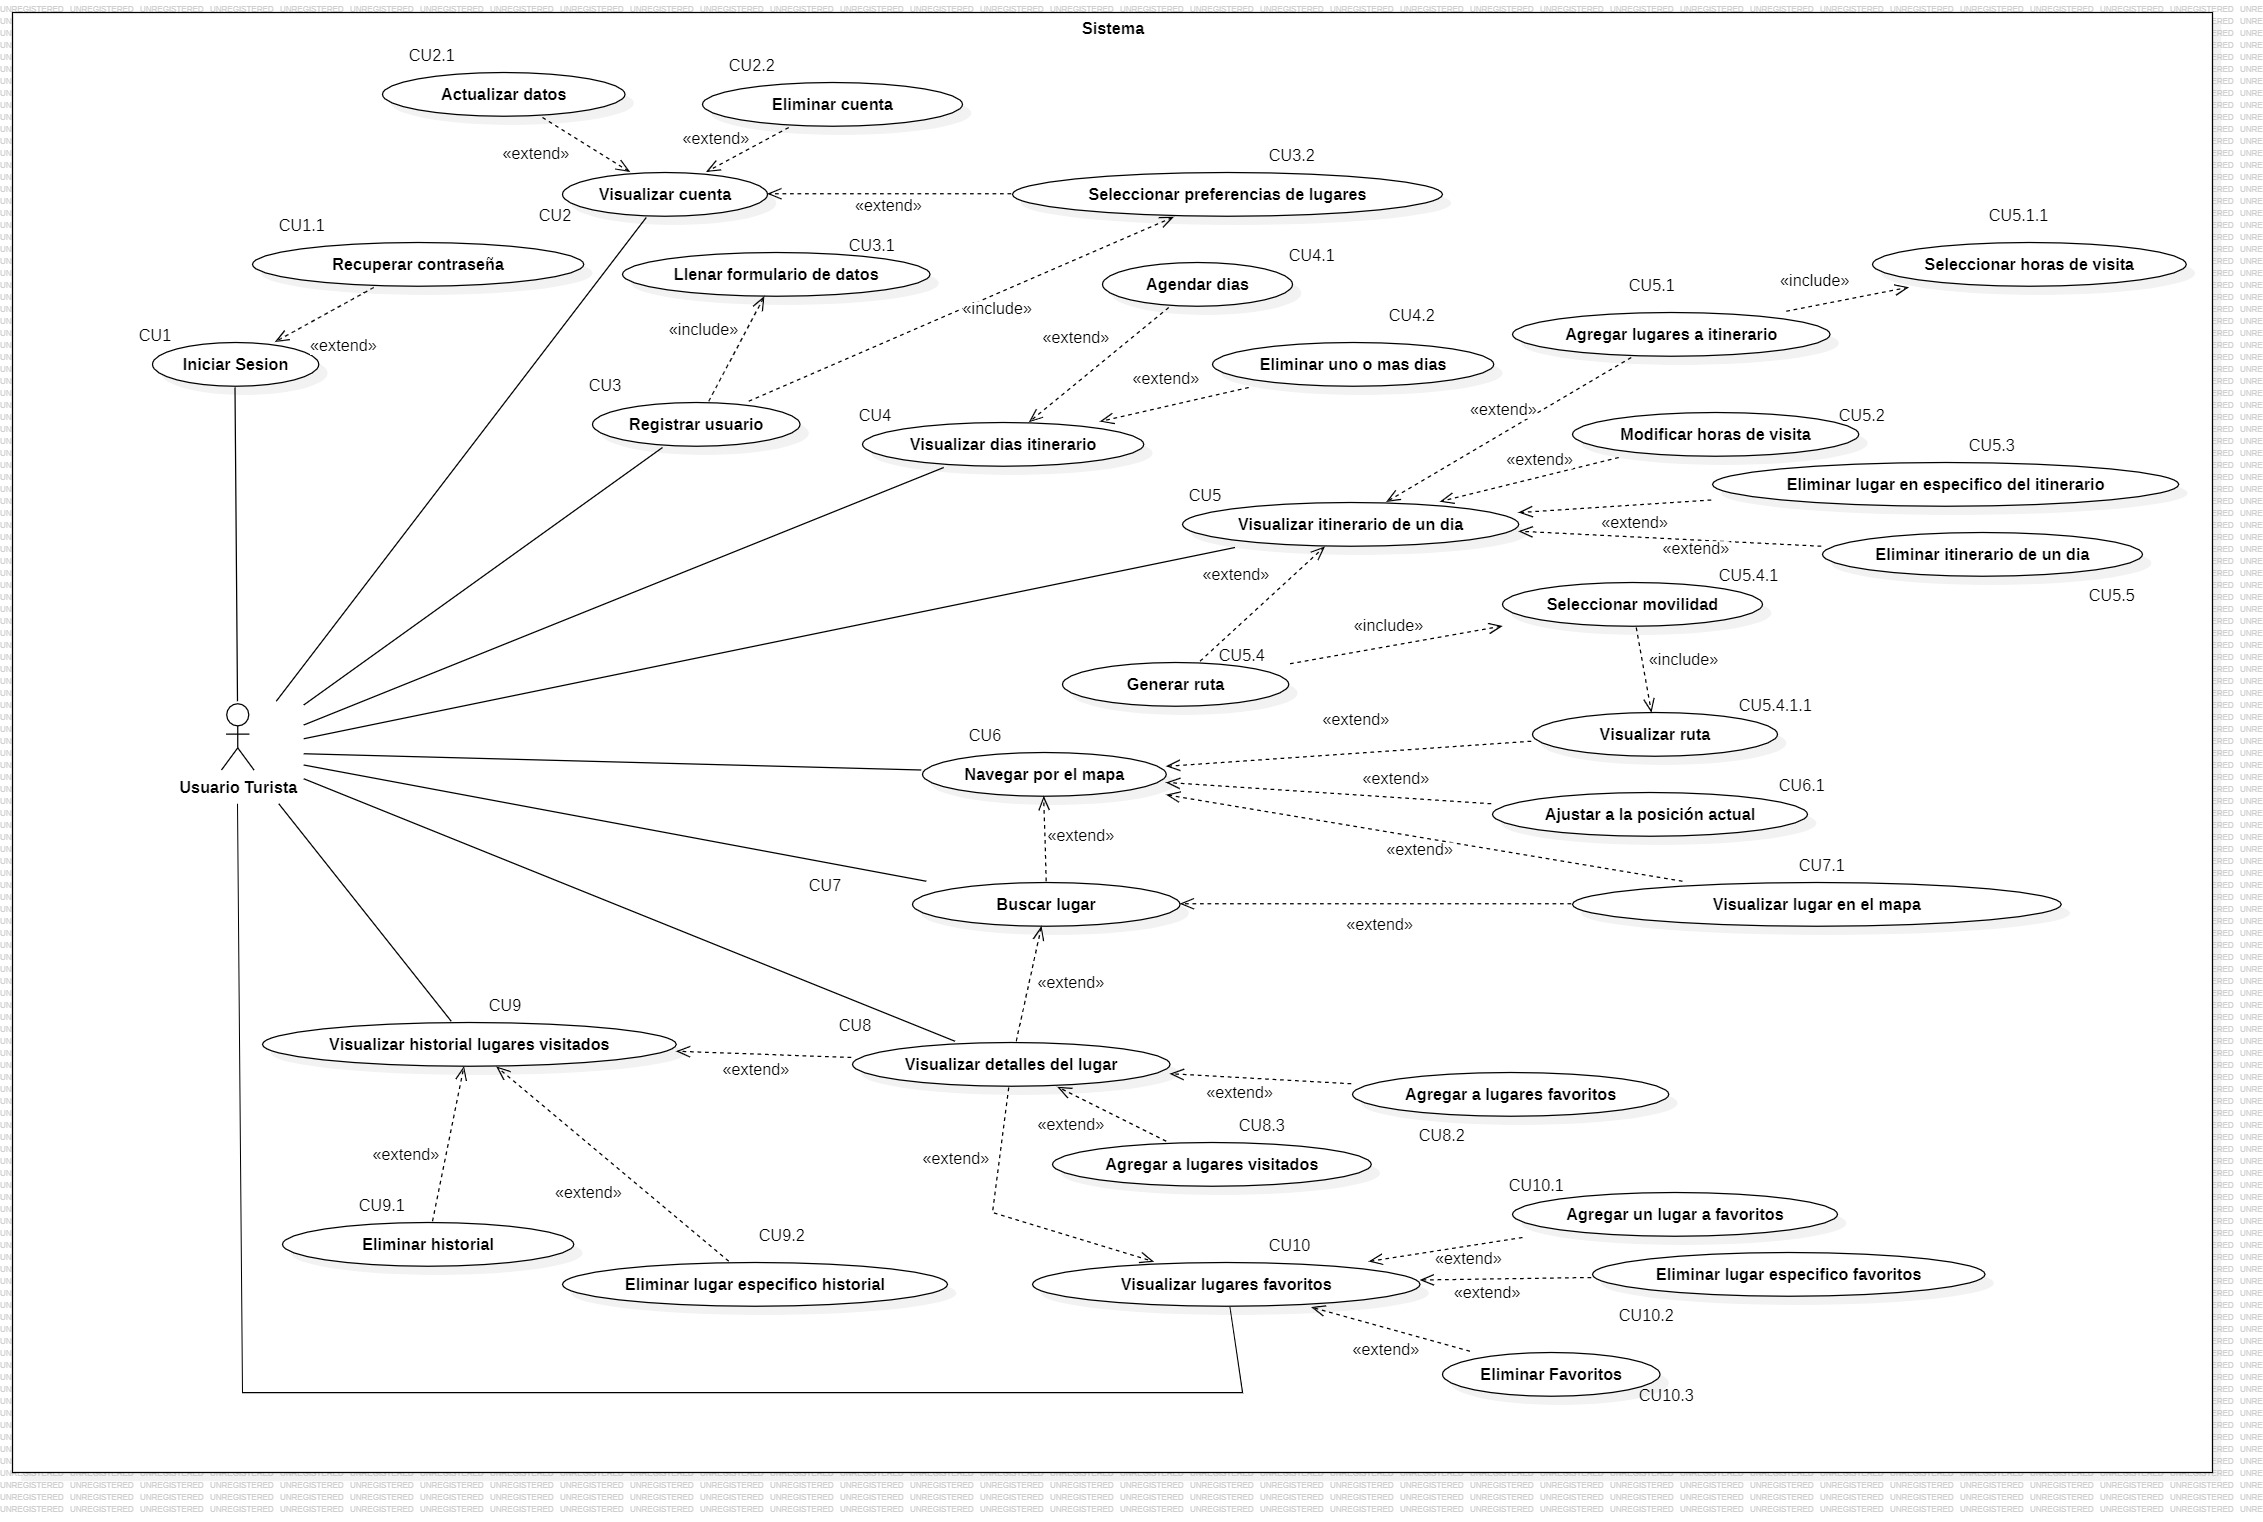
\includegraphics[width=16.5cm]{entregable final/caso_usoSA.jpg}
        \caption{Diagrama de Caso de Uso}
        \label{fig:enter-label}
    \end{figure}
    
\section{\textcolor{azul}{Definición de actores propuestos}}
\textbf{Usuario Admin}\\
Es el usuario que gestionara  el sistema cuyas principales funciones son getsionar y suspendercuentas de los turistas.\\
\vspace{.5cm}
\textbf{Usuario Turista}\\
Es el usuario que interactua con el sistema, es decir, el cliente de nuestra aplicacion, sus principales caracteristicas son creacion de cuentas para poder acceder al sistema, iniciar sesión en el sistema, visualizar su ubicacion en un mapa, poder visualizar sus datos de usuario, generar un itinerario de su ruta turistica, contar con un historial de los sitios que ha visitado, poder tener un apartado de favoritos, cerrar sesión, organizar sus horarios. 

%ARCHIVO DE PANTALLAS
\section{\textcolor{azul}{Prototipo no funcional}}
%jony
\begin{figure}[h]
    \begin{minipage}{0.4\textwidth}
        \centering
        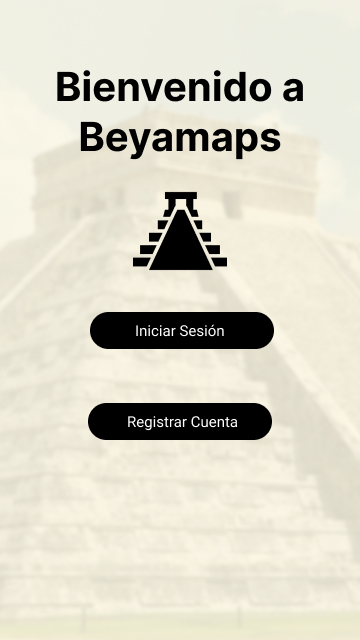
\includegraphics[width=.7\linewidth]{Pantallas Prototipo3/IU01 Pantalla incial.jpg}
        \caption{IU01 Pantalla incial}
    \end{minipage}
    
    \begin{minipage}{0.4\textwidth}
        \centering
        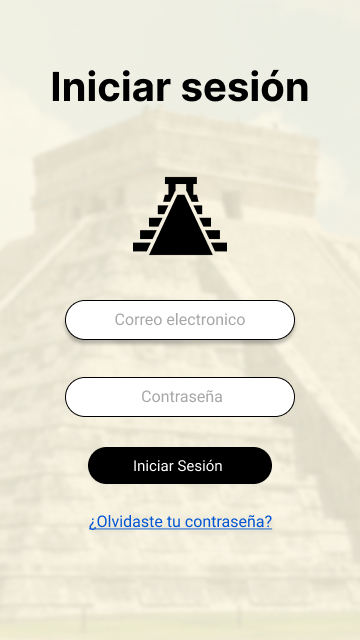
\includegraphics[width=.7\linewidth]{Pantallas Prototipo3/IU02 Pantalla Iniciar sesion.jpg}
        \caption{IU02 Pantalla Iniciar sesion}
    \end{minipage}%
\end{figure}

\begin{figure}[h]
    \begin{minipage}{0.5\textwidth}
        \centering
        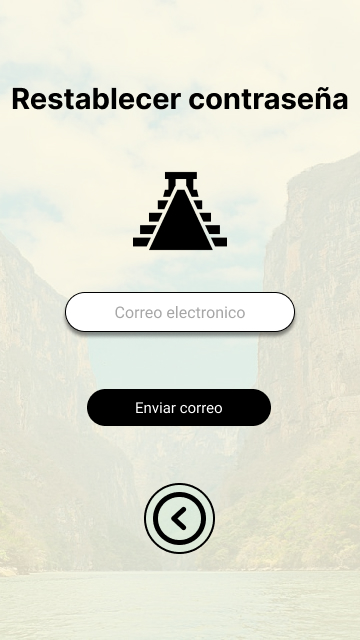
\includegraphics[width=.7\linewidth]{Pantallas Prototipo3/IU03 Pantalla correo restablecimiento.jpg}
        \caption{IU03 Pantalla correo restablecimiento.}
    \end{minipage}
    
    \begin{minipage}{0.5\textwidth}
        \centering
        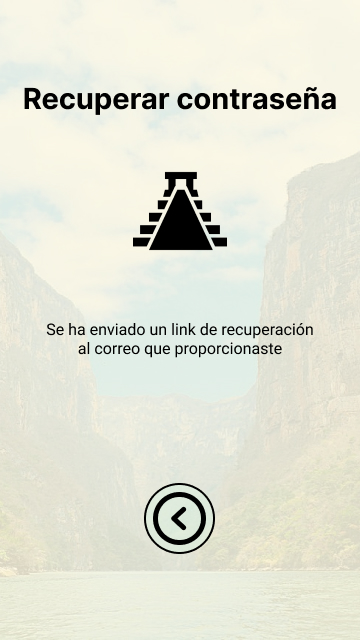
\includegraphics[width=.7\linewidth]{Pantallas Prototipo3/IU04 Pantalla link de recuperacion.jpg}
        \caption{IU04 Pantalla link de recuperacion}
    \end{minipage}%
\end{figure}

\begin{figure}[h]
    \begin{minipage}{0.5\textwidth}
        \centering
        \includegraphics[width=.7\linewidth]{Pantallas Prototipo3/IU05-Reestablacer contraseña.jpg}
        \caption{IU05 Reestablacer contraseña}
    \end{minipage}
    
    \begin{minipage}{0.5\textwidth}
        \centering
        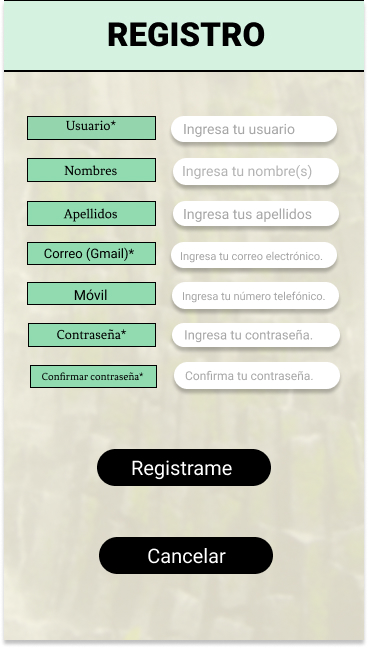
\includegraphics[width=.7\linewidth]{Pantallas Prototipo3/IU06-Registro de Cuenta.jpg}
        \caption{IU06 Registro de Cuenta}
    \end{minipage}%
\end{figure}

\begin{figure}[h]
    \begin{minipage}{0.5\textwidth}
        \centering
        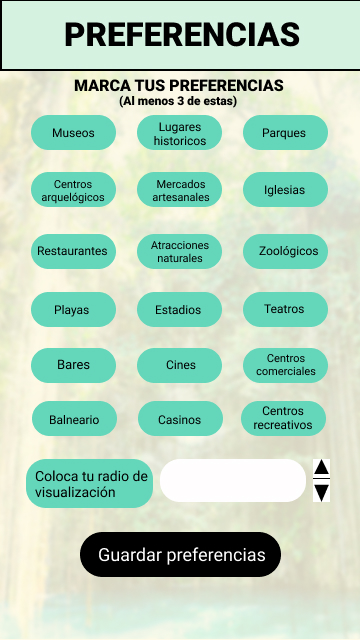
\includegraphics[width=.7\linewidth]{Pantallas Prototipo3/IU07-Preferencias del usuario.jpg}
        \caption{IU07 Preferencias del usuario}
    \end{minipage}
    
    \begin{minipage}{0.5\textwidth}
        \centering
        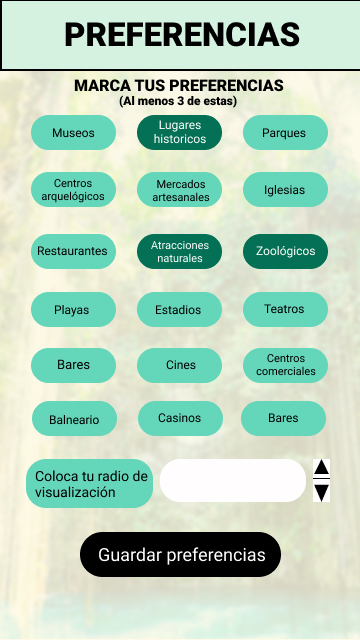
\includegraphics[width=.7\linewidth]{Pantallas Prototipo3/IU08-Preferencias del usuario.jpg}
        \caption{IU08 Preferencias del usuario seleccionadas}
    \end{minipage}%
\end{figure}

\begin{figure}[h]
    \begin{minipage}{0.5\textwidth}
        \centering
        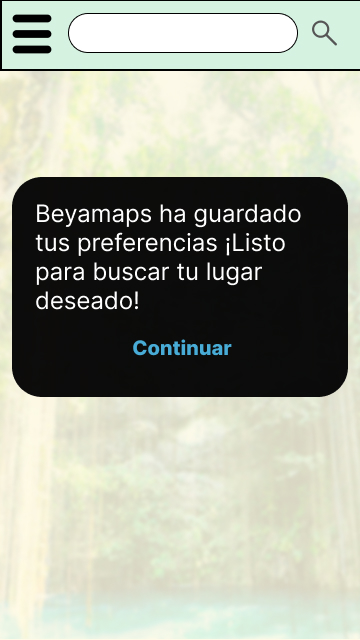
\includegraphics[width=.7\linewidth]{Pantallas Prototipo3/IU09Preferencias del usuario.jpg}
        \caption{IU09 Preferencias guardadas}
    \end{minipage}
    
    \begin{minipage}{0.5\textwidth}
        \centering
        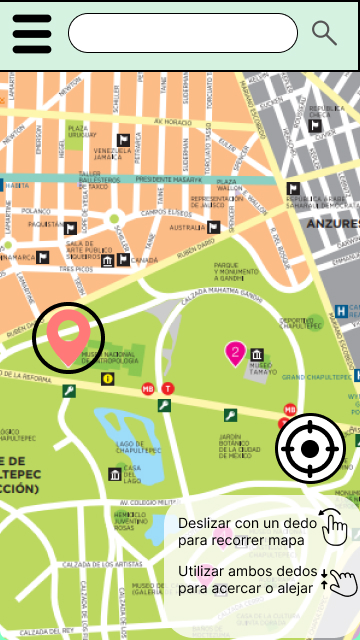
\includegraphics[width=.7\linewidth]{Pantallas Prototipo3/IU10 - Mapa principal.jpg}
        \caption{IU10 Mapa principal}
    \end{minipage}%
\end{figure}

\begin{figure}[h]
    \begin{minipage}{0.5\textwidth}
        \centering
        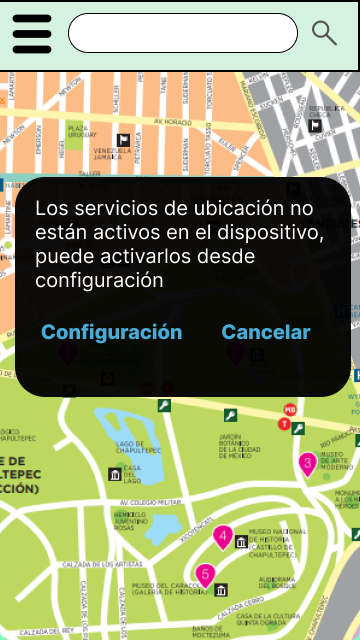
\includegraphics[width=.7\linewidth]{Pantallas Prototipo3/IU11 - Activar ubicacion.jpg}
        \caption{IU11 Activar ubicacion}
    \end{minipage}
%fin jony
%inicio Dario
    \begin{minipage}{0.5\textwidth}
        \centering
        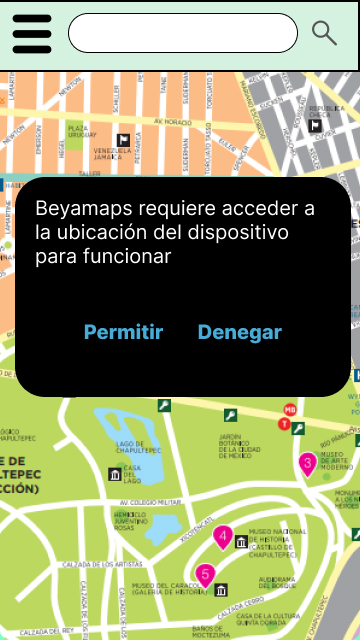
\includegraphics[width=.7\linewidth]{Pantallas Prototipo3/IU12 Pantalla Acceso Ubicacion.jpg}
        \caption{IU 12 Pantalla Acceso Ubicación}
    \end{minipage}%
\end{figure}

\begin{figure}[h]
    \begin{minipage}{0.5\textwidth}
        \centering
        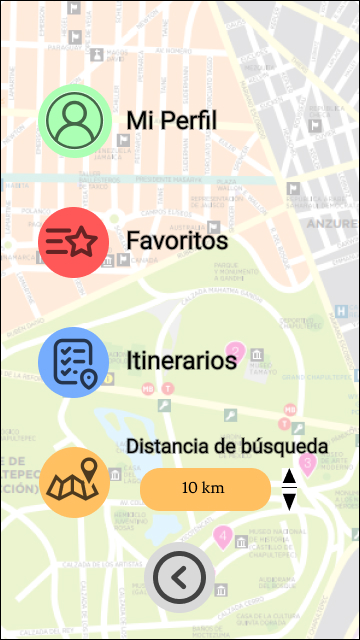
\includegraphics[width=.7\linewidth]{Pantallas Prototipo3/IU13 Pantalla Menu de Opciones.jpg}
        \caption{IU13 Pantalla Menu de Opciones}
    \end{minipage}
    
    \begin{minipage}{0.5\textwidth}
        \centering
        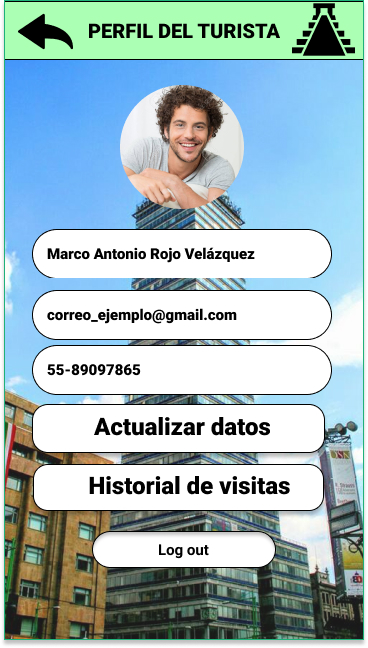
\includegraphics[width=.7\linewidth]{Pantallas Prototipo3/IU14 Pantalla de perfil.jpg}
        \caption{IU14 Pantalla Perfil}
    \end{minipage}%
\end{figure}

\begin{figure}[h]
    \begin{minipage}{0.5\textwidth}
        \centering
        \includegraphics[width=.7\linewidth]{Pantallas Prototipo3/IU15 Pantalla Validacion de Contraseña.jpg}
        \caption{IU15 Pantalla Validación de Contraseña}
    \end{minipage}
    
    \begin{minipage}{0.5\textwidth}
        \centering
        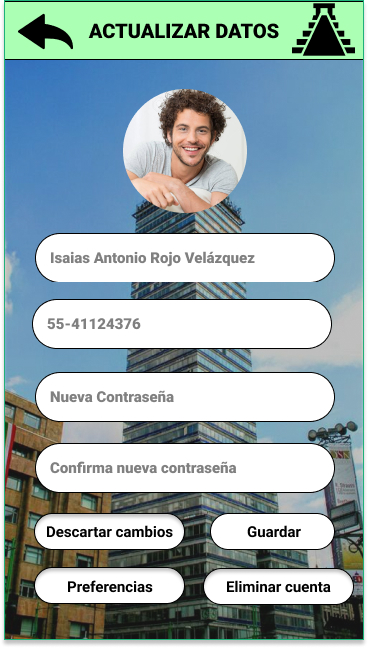
\includegraphics[width=.7\linewidth]{Pantallas Prototipo3/IU16 Pantalla de seleccionar el dato a editar.jpg}
        \caption{IU16 Pantalla Seleccionar Datos a Editar}
    \end{minipage}%
\end{figure}

\begin{figure}[h]
    \begin{minipage}{0.5\textwidth}
        \centering
        \includegraphics[width=.7\linewidth]{Pantallas Prototipo3/IU17 Pantalla Confirmación de guardado.jpg}
        \caption{IU17 Pantalla Confirmación de Guardado}
    \end{minipage}
    
    \begin{minipage}{0.5\textwidth}
        \centering
        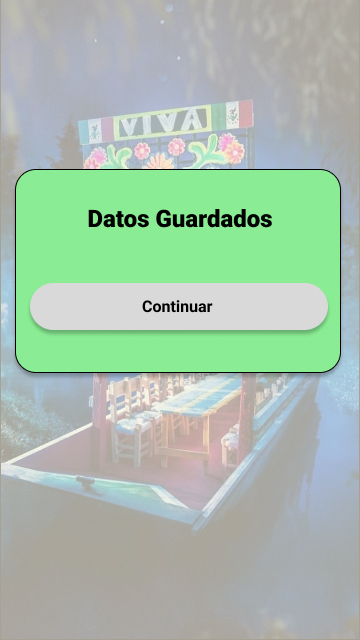
\includegraphics[width=.7\linewidth]{Pantallas Prototipo3/IU18 Pantalla Datos Guardados.jpg}
        \caption{IU18 Pantalla Datos Guardados}
    \end{minipage}%
\end{figure}

\begin{figure}[h]
    \begin{minipage}{0.5\textwidth}
        \centering
        \includegraphics[width=.7\linewidth]{Pantallas Prototipo3/IU19 Pantalla Ventana de confirmación de eliminar cuenta.jpg}
        \caption{IU19 Pantalla Ventana Confirmación Eliminar Cuenta}
    \end{minipage}
    
    \begin{minipage}{0.5\textwidth}
        \centering
        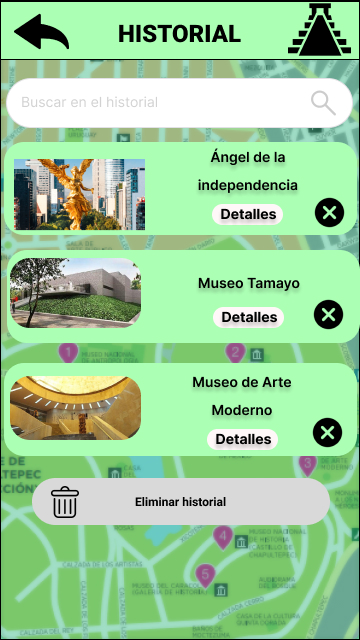
\includegraphics[width=.7\linewidth]{Pantallas Prototipo3/IU20 Pantalla Historial.jpg}
        \caption{IU20 Pantalla Historial}
    \end{minipage}%
\end{figure}

\begin{figure}[h]
    \begin{minipage}{0.5\textwidth}
        \centering
        \includegraphics[width=.7\linewidth]{Pantallas Prototipo3/IU21 Ventana confirmación eliminar.jpg}
        \caption{IU21 Pantalla Ventana Confirmación Eliminar}
    \end{minipage}
    
    \begin{minipage}{0.5\textwidth}
        \centering
        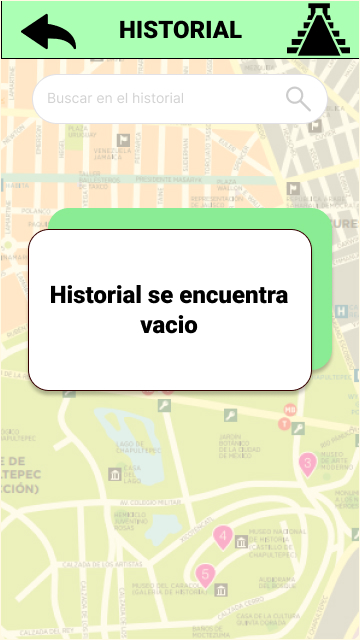
\includegraphics[width=.7\linewidth]{Pantallas Prototipo3/IU22 Historial vacio.jpg}
        \caption{IU22 Pantalla Historial Vacio}
    \end{minipage}%
\end{figure}
%fin dario
%inicio leo
\begin{figure}[h]
    \begin{minipage}{0.5\textwidth}
        \centering
        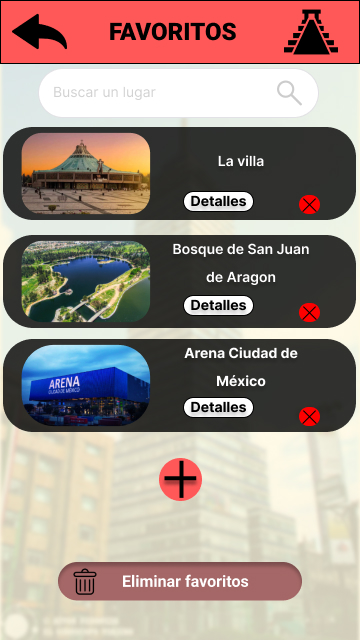
\includegraphics[width=.7\linewidth]{Pantallas Prototipo3/IU23 Pantalla Favoritos.jpg}
        \caption{IU23 Pantalla Favoritos}
    \end{minipage}
    
    \begin{minipage}{0.5\textwidth}
        \centering
        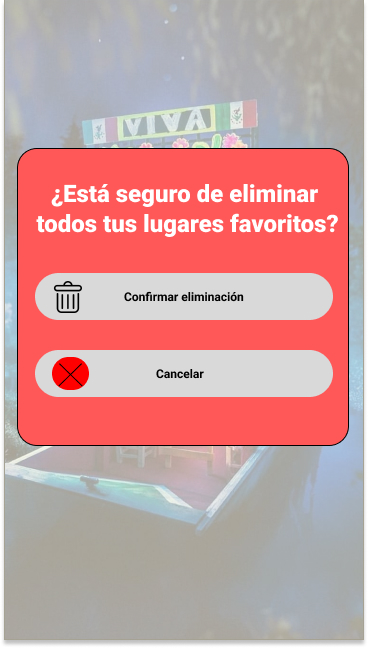
\includegraphics[width=.7\linewidth]{Pantallas Prototipo3/IU24 Pantalla Eliminacion favoritos.jpg}
        \caption{IU24 Pantalla Eliminacion favoritos}
    \end{minipage}%
\end{figure}

\begin{figure}[h]
    \begin{minipage}{0.5\textwidth}
        \centering
        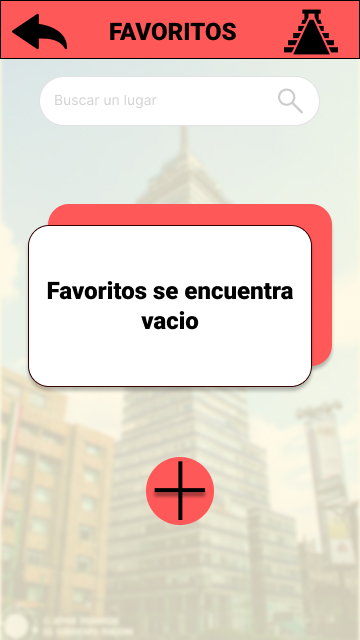
\includegraphics[width=.7\linewidth]{Pantallas Prototipo3/IU25 Pantalla Favoritos vacio.jpg}
        \caption{IU25 Pantalla Favoritos vacio}
    \end{minipage}
    
    \begin{minipage}{0.5\textwidth}
        \centering
        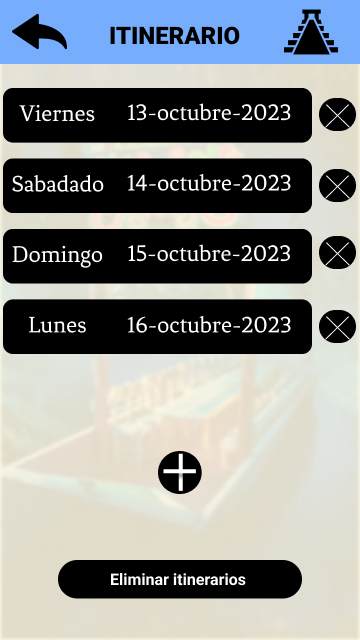
\includegraphics[width=.7\linewidth]{Pantallas Prototipo3/IU26 Pantalla Dias Itinerario.jpg}
        \caption{IU26 Pantalla Dias Itinerario}
    \end{minipage}%
\end{figure}

\begin{figure}[h]
    \begin{minipage}{0.5\textwidth}
        \centeringz
        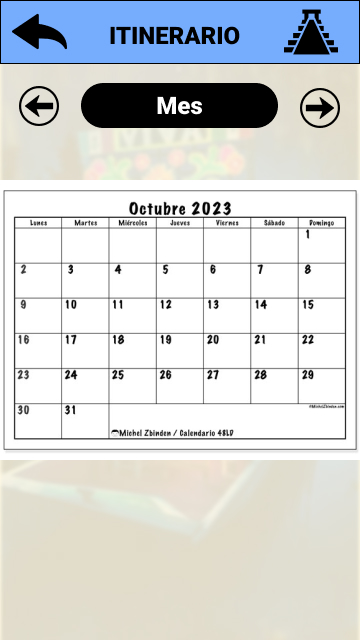
\includegraphics[width=.7\linewidth]{Pantallas Prototipo3/IU27 Pantalla Dia calendario.jpg}
        \caption{IU27 Pantalla Dia calendario}
    \end{minipage}
    
    \begin{minipage}{0.5\textwidth}
        \centering
        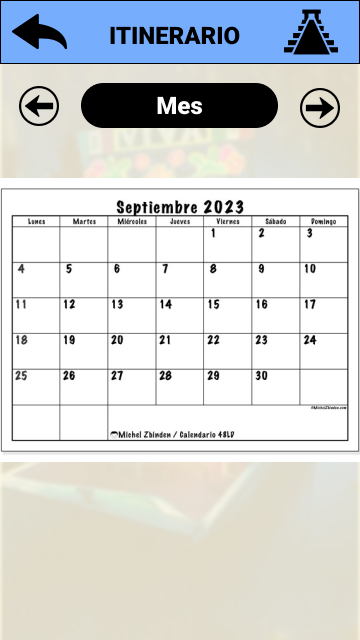
\includegraphics[width=.7\linewidth]{Pantallas Prototipo3/IU28 Pantalla Dia Mes Diferente.jpg}
        \caption{IU28 Pantalla Dia Mes Diferente}
    \end{minipage}%
\end{figure}

\begin{figure}[h]
    \begin{minipage}{0.5\textwidth}
        \centering
        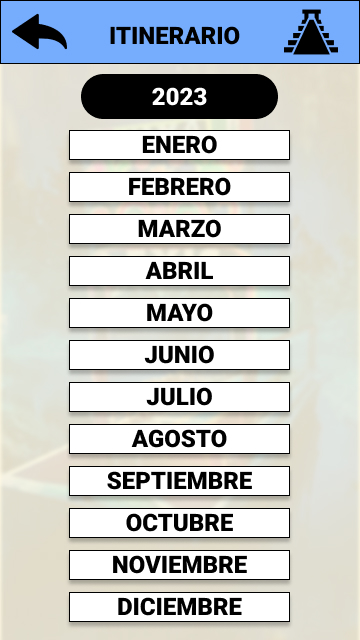
\includegraphics[width=.7\linewidth]{Pantallas Prototipo3/IU29 Pantalla Mes Calendario.jpg}
        \caption{IU29 Pantalla Mes Calendario}
    \end{minipage}
    
    \begin{minipage}{0.5\textwidth}
        \centering
        \includegraphics[width=.7\linewidth]{Pantallas Prototipo3/IU30 Pantalla Año Calendario.jpg}
        \caption{IU30 Pantalla Año Calendario}
    \end{minipage}%
\end{figure}

\begin{figure}[h]
    \begin{minipage}{0.5\textwidth}
        \centering
        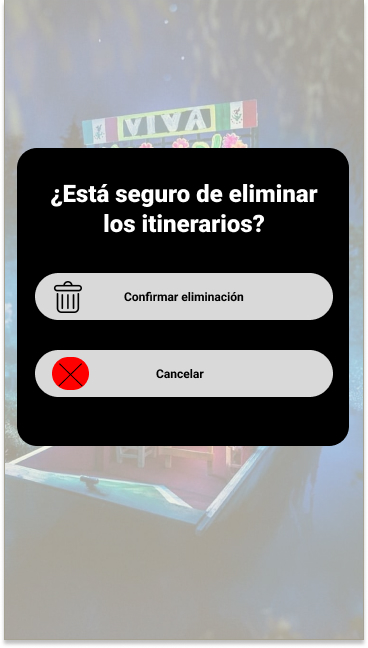
\includegraphics[width=.7\linewidth]{Pantallas Prototipo3/IU31 Pantalla Eliminar Itinerario.jpg}
        \caption{IU31 Pantalla Eliminar Itinerario}
    \end{minipage}
    
    \begin{minipage}{0.5\textwidth}
        \centering
        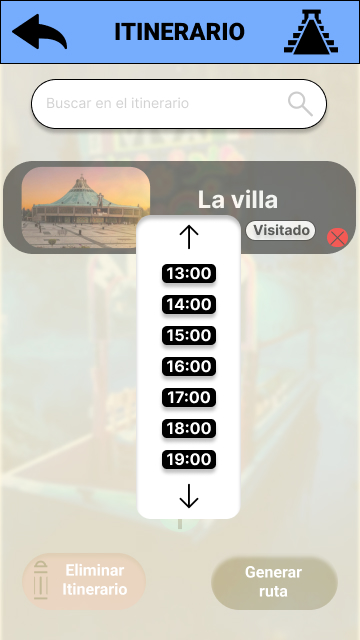
\includegraphics[width=.7\linewidth]{Pantallas Prototipo3/IU32 Pantalla Horas Lugar.jpg}
        \caption{IU32 Pantalla Horas Lugar}
    \end{minipage}%
\end{figure}

\begin{figure}[h]
    \begin{minipage}{0.5\textwidth}
        \centering
        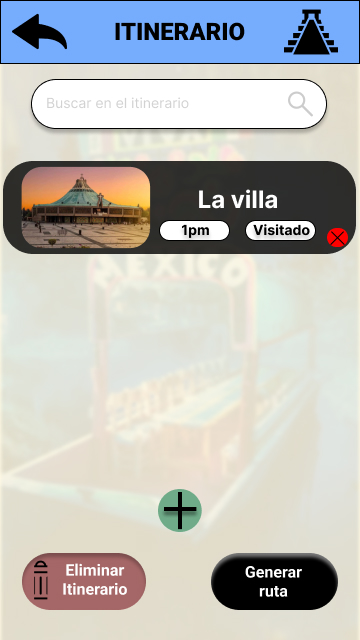
\includegraphics[width=.7\linewidth]{Pantallas Prototipo3/IU33 Pantalla Itinerario Dia.jpg}
        \caption{IU33 Pantalla Itinerario Dia}
    \end{minipage}
%fin leo
%inicio said
    \begin{minipage}{0.5\textwidth}
        \centering
        \includegraphics[width=.7\linewidth]{Pantallas Prototipo3/IU34-Ventana confirmación eliminar itinerario.jpg}
        \caption{IU34 Pantalla confirmación eliminar itinerario}
    \end{minipage}%
\end{figure}

\begin{figure}[h]
    \begin{minipage}{0.5\textwidth}
        \centering
        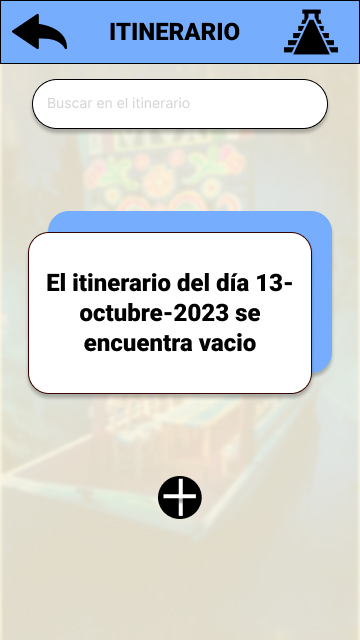
\includegraphics[width=.7\linewidth]{Pantallas Prototipo3/IU35-itinerario vacio en el dia x-x-x.jpg}
        \caption{IU35 Pantalla itinerario vacio en el dia x-x-x}
    \end{minipage}
    
    \begin{minipage}{0.5\textwidth}
        \centering
        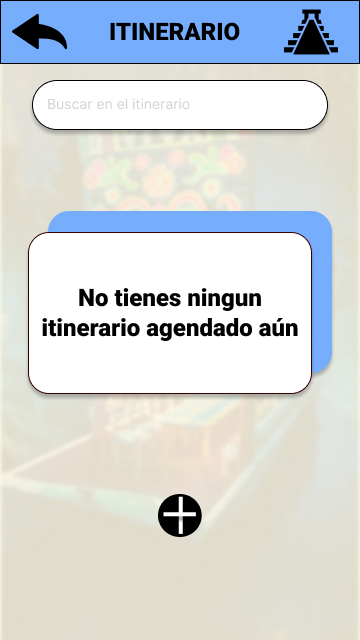
\includegraphics[width=.7\linewidth]{Pantallas Prototipo3/IU36-dias del itineraio vacio.jpg}
        \caption{IU36 Pantalla dias del itineraio vacio}
    \end{minipage}%
\end{figure}

\begin{figure}[h]
    \begin{minipage}{0.5\textwidth}
        \centering
        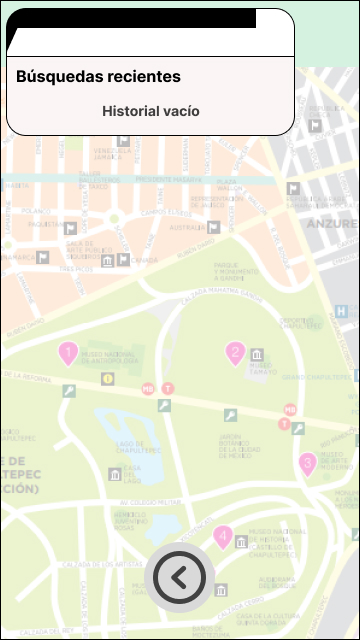
\includegraphics[width=.7\linewidth]{Pantallas Prototipo3/IU37-Historial de Búsqueda Vacío.jpg}
        \caption{IU37 Pantalla Historial de Búsqueda Vacío}
    \end{minipage}
    
    \begin{minipage}{0.5\textwidth}
        \centering
        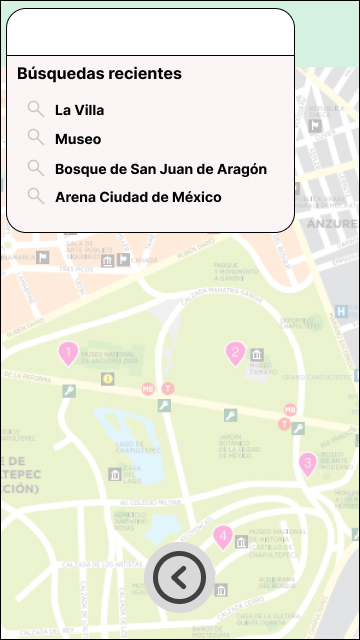
\includegraphics[width=.7\linewidth]{Pantallas Prototipo3/IU38-Buscar un lugar.jpg}
        \caption{IU38 Pantalla Buscar un lugar}
    \end{minipage}%
\end{figure}

\begin{figure}[h]
    \begin{minipage}{0.5\textwidth}
        \centering
        \includegraphics[width=.7\linewidth]{Pantallas Prototipo3/IU39-Búsqueda de un lugar.jpg}
        \caption{IU39 Pantalla Búsqueda de un lugar}
    \end{minipage}
    
    \begin{minipage}{0.5\textwidth}
        \centering
        \includegraphics[width=.7\linewidth]{Pantallas Prototipo3/IU40-Búsqueda sin resultado.jpg}
        \caption{IU40 Pantalla Búsqueda sin resultado}
    \end{minipage}%
\end{figure}

\begin{figure}[h]
    \begin{minipage}{0.5\textwidth}
        \centering
        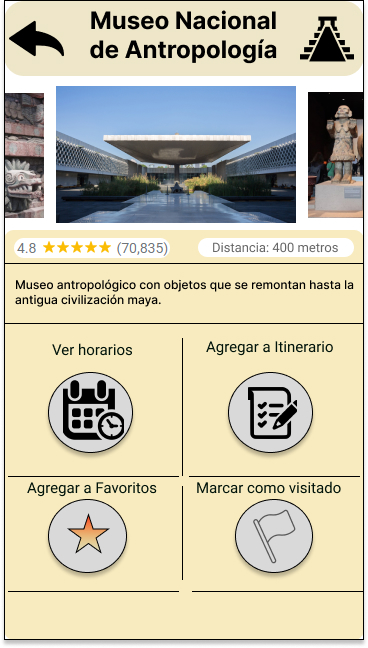
\includegraphics[width=.7\linewidth]{Pantallas Prototipo3/IU41-Detalles del lugar.jpg}
        \caption{IU41 Pantalla Detalles del lugar}
    \end{minipage}
    
    \begin{minipage}{0.5\textwidth}
        \centering
        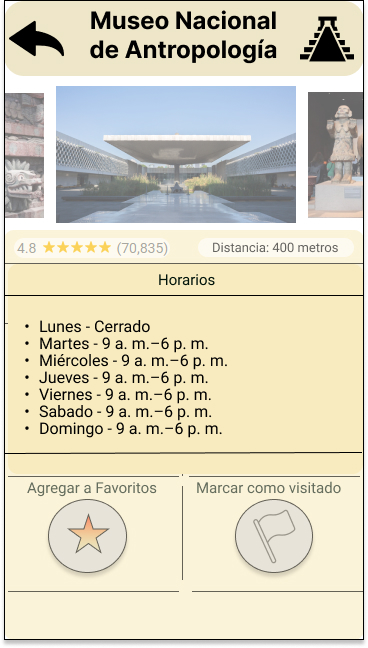
\includegraphics[width=.7\linewidth]{Pantallas Prototipo3/IU42-Ver horario.jpg}
        \caption{IU42 Pantalla Ver horario}
    \end{minipage}%
\end{figure}

\begin{figure}[h]
    \begin{minipage}{0.5\textwidth}
        \centering
        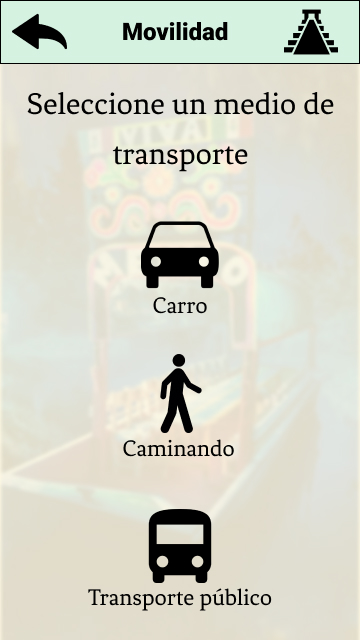
\includegraphics[width=.7\linewidth]{Pantallas Prototipo3/IU43-Movilidad.jpg}
        \caption{IU43 Pantalla Movilidad}
    \end{minipage}
    
    \begin{minipage}{0.5\textwidth}
        \centering
        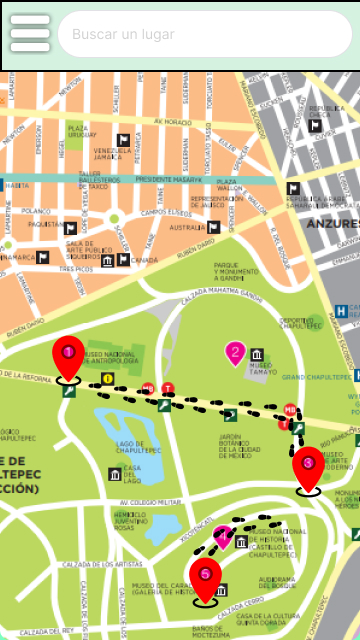
\includegraphics[width=.7\linewidth]{Pantallas Prototipo3/IU44-Ruta generada.jpg}
        \caption{IU44 Pantalla Ruta generada}
    \end{minipage}%
\end{figure}

%ARCHIVO DESCRIPCION CASOS DE USO

\section{{Descripción casos de uso}}

%--------------------------Inicia otro caso de uso (javier)--------------------------------------------------------------%

\subsection{\textcolor{blue}{CU 1.1 Restablecer contraseña}}

\subsubsection{\textcolor{blue}{Resumen}}
Se brindara al usuario la posibilidad de recuperar sus datos para acceder al sistenma en caso de haberlos olvidado o perdido.
\subsubsection{\textcolor{blue}{Descripción}}
\begin{tabularx}{16cm}{||l|X||}
	\hline
	\multicolumn{2}{||c||}{Caso de Uso: Reestablecer contraseña } \\
	\hline
	\multicolumn{2}{||c||}{\textcolor{blue}{Resumen de atributos}} \\
	\hline
	{Autor:} & Zamarrón Ramírez Javier \\
    \hline
	{Actor:} & Usuario turista\\
	\hline
	{Próposito:} & Permitir al usuario restablecer contraseña\\
	\hline
	{Entradas:} &  Se escribe desde la pantalla del celular el correo electrónico del usuario. \\
	\hline
	{Salidas:} & Se envía el mensaje de correo electrónico de recuperación de contraseña \\
	\hline
	{Precondiciones:} & Debe existir una cuenta activa en el sistema con el correo electronico.\\ 
	\hline
	{Postcondiciones:} & Se elimina la cuenta del usuario, por lo que el sistema deja de almacenar su informacion.\\
	\hline
	{Errores:} &\begin{minipage}{1\linewidth}
        \begin{enumerate}
            \item Cuando el correo electrónico no es válido, se mostrará el mensaje de alerta 1.
            \item Cuando el correo electrónico no está asociado a una cuenta activa, se mostrará el mensaje de alerta 2.
            \item Cuando las contraseñas no son iguales, se mostrará el mensaje de alerta 3.
            \item Cuando la contraseña no cumple con la regla de negocio 5, se mostrará el mensaje de alerta 4.
        \end{enumerate}
    \end{minipage} \\
	\hline
	{Tipo:} & Reunion interna\\
	\hline
	{Fuente:} & {-} \\
	\hline
	{Observaciones:} & {-} \\
	\hline
\end{tabularx}

\pagebreak
\subsubsection{\textcolor{blue}{Trayectorias del caso de uso}}
\textbf{Trayectoria Principal}
    \begin{enumerate}
    \item 
\includegraphics[width=0.0150\textwidth]{Figuras/persona.png} presiona la leyenda olvidaste tu contraseña? en la pantalla \textcolor{blue}{Iniciar sesion}.
    \item 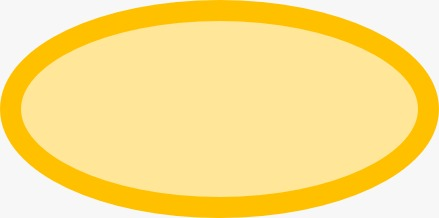
\includegraphics[width=0.0500\textwidth]{Figuras/sistema.png} muestra la pantalla Recuperar contraseña.
    \item 
\includegraphics[width=0.0150\textwidth]{Figuras/persona.png} solicita recuperar los datos de su cuenta oprimiendo ¿Olvidaste tu contraseña? de la pantalla \textcolor{blue}{Iniciar sesion}.
     \item 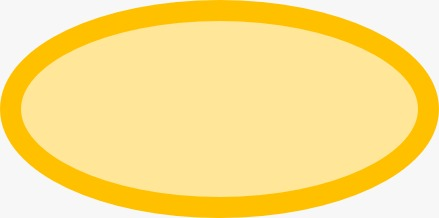
\includegraphics[width=0.0500\textwidth]{Figuras/sistema.png} solicita ingresar el correo electronico asociado a la cuenta de la que se desea reestablecer la contraseña mostrando la pantalla \textcolor{blue}{Recuperacion de contraseña} [Trayectoria A].
    \item 
\includegraphics[width=0.0150\textwidth]{Figuras/persona.png} ingresa el correo electronico .
    \item \includegraphics[width=0.0150\textwidth]{Figuras/persona.png} solicita reestablecer la contraseña de su cuenta oprimiendo el boton de enviar correo.
    \item \includegraphics[width=0.0500\textwidth]{Figuras/sistema.png} verifica que el correo electronico sea valido. [Trayectoria B]
    \item \includegraphics[width=0.0500\textwidth]{Figuras/sistema.png} verifica que el correo electronico este asociado a una cuenta activa. [Trayectoria C].
    \item \includegraphics[width=0.0500\textwidth]{Figuras/sistema.png} genera y registra el token de restablecimiento de contraseña.
    \item \includegraphics[width=0.0500\textwidth]{Figuras/sistema.png} envia por correo electronico el mensaje \textcolor{blue}{E-mail1 Correo recuperación de contraseña} .
    \item \includegraphics[width=0.0150\textwidth]{Figuras/persona.png} accede al enlace enviado por correo electrónico.
    \item \includegraphics[width=0.0500\textwidth]{Figuras/sistema.png} recibe la solicitud del usuario para restablecer contraseña.
    \item \includegraphics[width=0.0500\textwidth]{Figuras/sistema.png} verifica que el token de la cuenta sea valido.
    \item \includegraphics[width=0.0500\textwidth]{Figuras/sistema.png} verifica que el token de la cuenta sea valido.
    \item \includegraphics[width=0.0500\textwidth]{Figuras/sistema.png} muestra al usuario la pantalla de Restablecer contraseña.
    \item \includegraphics[width=0.0150\textwidth]{Figuras/persona.png} escribe sus contraseñas y presiona el boton Guardar contraseña.
    \item \includegraphics[width=0.0500\textwidth]{Figuras/sistema.png} verifica si ambas contraseñas son iguales. [Trayectoria D]
    \item \includegraphics[width=0.0500\textwidth]{Figuras/sistema.png} verifica si la contraseña proporcionada cumple con los requisitos mencionados en la regla de negocio 5. [Trayectoria E]
    \item \includegraphics[width=0.0500\textwidth]{Figuras/sistema.png} elimina el token de restablecimiento de contraseña generado.
    \item \includegraphics[width=0.0500\textwidth]{Figuras/sistema.png} actualiza la contraseña del usuario.
    \item \includegraphics[width=0.0500\textwidth]{Figuras/sistema.png} muestra la pantalla Recuperacion de contraseña (exitoso) y se redirecciona a pantalla Iniciar sesion.\\
    - - - Fin de caso de uso
\end{enumerate}

\textbf{Trayectoria A}\\
Condición : \includegraphics[width=0.0150\textwidth]{Figuras/persona.png} desea cancelar el cambio de contraseña
\begin{itemize}
    \item \includegraphics[width=0.0150\textwidth]{Figuras/persona.png} oprime el boton de regresar.
     \item \includegraphics[width=0.0500\textwidth]{Figuras/sistema.png} muestra la pantalla Iniciar sesion.
    \item Termina el caso de uso.\\
    - - - Fin de trayectoria
\end{itemize}
\textbf{Trayectoria B}\\
Condición :  \includegraphics[width=0.0150\textwidth]{Figuras/persona.png} no escribio un correo valido.
\begin{itemize}
    \item \includegraphics[width=0.0500\textwidth]{Figuras/sistema.png} muestra en la pantalla Recuperacion de contraseña el mensaje alerta 1.
    \item Continua en el paso 5\\
    - - - Fin de trayectoria
\end{itemize}
\textbf{Trayectoria C}\\
Condición : \includegraphics[width=0.0150\textwidth]{Figuras/persona.png} escribio un correo electronico que no esta asociado a una cuenta activa.
\begin{itemize}
    \item \includegraphics[width=0.0500\textwidth]{Figuras/sistema.png} muestra en la pantalla Recuperacion de contraseña el mensaje alerta 2.
    \item Continua en el paso 3\\
    - - - Fin de trayectoria
\end{itemize}
\textbf{Trayectoria D}\\
Condición : Las contraseñas escritas por \includegraphics[width=0.0150\textwidth]{Figuras/persona.png} no son iguales.
\begin{itemize}
    \item  \includegraphics[width=0.0500\textwidth]{Figuras/sistema.png} muestra en la pantalla restablecer contraseña el mensaje alerta 3.
    \item Continua en el paso 14.\\
    - - - Fin de trayectoria
\end{itemize}
\textbf{Trayectoria E}\\
Condición : La contraseña escrita por el \includegraphics[width=0.0150\textwidth]{Figuras/persona.png} no cumple con la regla de negocio 5.
\begin{itemize}
    \item \includegraphics[width=0.0500\textwidth]{Figuras/sistema.png} muestra en la pantalla restablecer contraseña el mensaje alerta 4.
    \item Continua en el paso 14.\\
    - - - Fin de trayectoria
\end{itemize}
\subsubsection{\textcolor{blue}{Pantalla IU3 y IU4}}

    \begin{figure}[htb]
        \centering
        \includegraphics[width= 5cm]{Pantallas Prototipo3/IU03 Pantalla correo restablecimiento.jpg}
        \caption{IU03 Recuprar contraseña}
        \label{fig:enter-label}
    \end{figure}
    \begin{figure}[htb]
        \centering
        \includegraphics[width= 5cm]{Pantallas Prototipo3/IU05-Reestablacer contraseña.jpg}
        \caption{IU04 Escribir contraseña nueva}
        \label{fig:enter-label}
    \end{figure}

%---------------------------------------Finaliza caso de uso (javier)%---------------------------------------------------
%-----------------------------------------------------------------------------------------------------------------------

















%--------------------------Inicia otro caso de uso (said)--------------------------------------------------------------%

\subsection{\textcolor{blue}{CU 2.2 Eliminar cuenta}}

\subsubsection{\textcolor{blue}{Resumen}}
Se brinda al usuario la posibilidad de poder eliminar su cuenta, además se necesita ingresar la contraseña como metodo de validacion.
\subsubsection{\textcolor{blue}{Descripción}}
\begin{tabularx}{16cm}{||l|X||}
	\hline
	\multicolumn{2}{||c||}{Caso de Uso: } \\
	\hline
	\multicolumn{2}{||c||}{\textcolor{blue}{Resumen de atributos}} \\
	\hline
	{Autor:} & Estrada Yepez Omar Said \\
    \hline
	{Actor:} & Usuario turista\\
	\hline
	{Próposito:} & Que el sistema permita al usuario eliminar su cuenta en cualquier momento si asi lo desea.\\
	\hline
	{Entradas:} &  Boton con el nombre de Actualizar datos. \\
    &Se ingresa la contraseña del usuario\\
    &Se ingresa la confirmacion de la contraseña del usuario.\\
    &Boton para validar contraseñas\\
    &Boton de confirmacion de eliminar\\
	\hline
	{Salidas:} & En la pantalla se mostrara el mensaje "Su cuenta fue eliminada con exito"\\
	\hline
	{Precondiciones:} & Debe existir una cuenta activa en el sistema con el correo electronico.\\ 
	\hline
	{Postcondiciones:} & Se elimina la cuenta del usuario, por lo que el sistema deja de almacenar su informacion.\\
	\hline
	{Errores:} & Cuando se proporciona la contraseña no coincide con el formato requerido de una contraseña. \\
    &No coincide la contraseña con la confirmacion de contraseña, se muestra el mensaje Las contraseñas deben ser iguales.\\
	\hline
	{Tipo:} & -\\
	\hline
	{Fuente:} & Reunion interna \\
	\hline
	{Observaciones:} & {-} \\
	\hline
\end{tabularx}

\pagebreak
\subsubsection{\textcolor{blue}{Trayectorias del caso de uso}}
\textbf{Trayectoria Principal}
    \begin{enumerate}
        \item \includegraphics[width=0.0150\textwidth]{Figuras/persona.png} El usuario solicita modificar datos oprimiendo el boton \includegraphics[width=0.2\textwidth]{ComponentesCU/AD.png}  de la Pantalla de perfil.
        \item \includegraphics[width=0.0500\textwidth]{Figuras/sistema.png} Muestra la Pantalla de seleccionar el dato a editar, mostrando en la parte inferior derecha el boton \includegraphics[width=0.2\textwidth]{ComponentesCU/img.png}.
        \item \includegraphics[width=0.0150\textwidth]{Figuras/persona.png} Oprime el boton \includegraphics[width=0.2\textwidth]{ComponentesCU/img.png}.
         \item \includegraphics[width=0.0500\textwidth]{Figuras/sistema.png} Muestra la pantalla Validacion de contraseña para modificacion de datos.
        \item \includegraphics[width=0.0500\textwidth]{Figuras/sistema.png} Solicita la contraseña y confirmacion de contraseña del usuario.
        \item \includegraphics[width=0.0150\textwidth]{Figuras/persona.png} Ingresa su contraseña y su confirmacion de la misma.
        \item \includegraphics[width=0.0500\textwidth]{Figuras/sistema.png} Valida que las contraseñas sean iguales[Trayectoria A].
        \item \includegraphics[width=0.0150\textwidth]{Figuras/persona.png} Oprime el boton \includegraphics[width=0.2\textwidth]{ComponentesCU/img1.png} de la pantalla Validacion de contraseña para modificacion de datos.
        \item \includegraphics[width=0.0500\textwidth]{Figuras/sistema.png} Muestra la pantalla Ventana de confirmación de eliminar cuenta con el mensaje ¿Estas seguro de eliminar tu cuenta?
        \item \includegraphics[width=0.0150\textwidth]{Figuras/persona.png} Oprime el boton \includegraphics[width=0.25\textwidth]{ComponentesCU/img2.png} [Trayectoria B].
        \item \includegraphics[width=0.0500\textwidth]{Figuras/sistema.png} Elimina el perfil del usuario turista.
        \item \includegraphics[width=0.0500\textwidth]{Figuras/sistema.png} Muestra el mensaje Su cuenta fue eliminada con exito
    \end{enumerate}
---FIN DE LA TRAYECTORIA--\\\\
\textbf{Trayectoria A}
    \begin{enumerate}
        \item \includegraphics[width=0.0500\textwidth]{Figuras/sistema.png} Muestra en la pantalla Validacion de contraseña erronea para modificacion de datos el mensaje Las contraseñas deben ser iguales indicando al usuario que las contraseñas son diferentes.
        \item \includegraphics[width=0.0500\textwidth]{Figuras/sistema.png} Continua el paso 5 de la trayectoria principal.
    \end{enumerate}
---FIN DE LA TRAYECTORIA--\\\\
\textbf{Trayectoria B}
    \begin{enumerate}
        \item \includegraphics[width=0.0150\textwidth]{Figuras/persona.png} Oprime el boton \includegraphics[width=0.25\textwidth]{ComponentesCU/img3.png}
        \item \includegraphics[width=0.0500\textwidth]{Figuras/sistema.png} Muestra la Pantalla de perfil
    \end{enumerate}
---FIN DE LA TRAYECTORIA--
\newpage
\subsubsection{\textcolor{blue}{Pantalla IUXXX}}
\begin{figure}[htbp]
        \centering
        \includegraphics[width= 5cm]{Pantallas Prototipo3/IU14 Pantalla de perfil.jpg}
        \caption{Pantalla de perfil}
        \label{fig:enter-label}
\end{figure}
\begin{figure}[htbp]
    \centering
    \includegraphics[width= 5cm]{Pantallas Prototipo3/IU16 Pantalla de seleccionar el dato a editar.jpg}
    \caption{Pantalla de seleccionar el dato a editar}
    \label{fig:enter-label}
\end{figure}

\begin{figure}[htbp]
        \centering
        \includegraphics[width= 5cm]{Pantallas Prototipo3/IU15 Pantalla Validacion de Contraseña.jpg}
        \caption{Validacion de contraseña para modificacion de datos}
        \label{fig:enter-label}
\end{figure}

\begin{figure}[htbp]
        \centering
        \includegraphics[width= 5cm]{Pantallas Prototipo3/IU19 Pantalla Ventana de confirmación de eliminar cuenta.jpg}
        \caption{Ventana de confirmación de eliminar cuenta}
        \label{fig:enter-label}
        \vspace{200pt}
\end{figure}
\newpage
%---------------------------------------Finaliza caso de uso (Said)%---------------------------------------------------
%-----------------------------------------------------------------------------------------------------------------------

%--------------------------Inicia otro caso de uso (Fer)--------------------------------------------------------------%

\subsection{\textcolor{blue}{CU 3 Llenar formulario de datos}}
\subsubsection{\textcolor{blue}{Resumen}}
             Se permite al Usuario Turista llenar los formularios de datos con información personal, al momento en el que se registre; estos datos son esenciales para crear una cuenta de usuario. La privacidad y la seguridad de estos datos personales son fundamentales, garantizando que se utilizan de manera segura y conforme a las políticas de privacidad. El sistema proporciona una interfaz para el ingreso de los datos como el nombre, apellido, correo electrónico, número de teléfono, fecha de nacimiento y contraseña.
             
\subsubsection{Descripción} \\
            \begin{tabularx}{16cm}{||l|X||}
            	\hline
            	\multicolumn{2}{||c||}{Caso de Uso: : Llenar formulario de datos} \\
            	\hline
            	\multicolumn{2}{||c||}{\textcolor{blue}{Resumen de atributos}} \\
            	\hline
            	{Actor:} & {\textcolor{blue}{Usuario Turista}} \\
                \hline
                {Autor:} & {Murillo Mendoza María Fernanda} \\
            	\hline
            	{Próposito:} & {Permite al Usuario Turista llenar formularios de datos con su información personal, al momento en el que se registre.} \\
            	\hline
                 {Entradas:} & { \begin{itemize}
                        \item \textbf Se escribe desde el teclado un usuario válido
                        \item \textbf Se escribe desde el teclado un nombre y un apellido
                        \item \textbf Se escribe desde el teclado un correo electrónico Gmail
                        \item \textbf Se escribe desde el teclado numérico un teléfono móvil 
                        \item \textbf Se escribe desde el teclado una fecha de nacimiento
                        \item \textbf Se escribe desde el teclado una contraseña junto con su confirmación
                        
                    \end{itemize}
                  }\\ 
            	\hline
            	{Salidas:} & {Se mostrará la pantalla \textcolor{blue}{IU06 Pantalla Registro de Cuenta} con el mensaje \textcolor{blue}{MSJ Registro Exitoso} }\\
            	\hline
            	{Precondiciones:} & {Contar con un correo electrónico en Gmail}\\\\
            	\hline
            	{Postcondiciones:} & { 
             \begin{itemize}
                        \item \textbf El usuario podrá acceder al apartado beyamaps.
                        \item \textbf El usuario podrá ver su itinerario.
                        \item \textbf El usuario podrá marcar sus preferencias.
                        \item \textbf El usuario podrá modificar sus datos personales en un futuro.
                        \item \textbf El usuario podrá ver su historial.
                        \item \textbf El usuario podrá agregar y eliminar sus lugares favoritos.
                        \end{itemize}
                } \\
                    \hline
        \end{tabularx}
                  \newpage
                  \begin{tabularx}{16cm}{||l|X||}
                  \hline
            	{Errores:} & { \begin{itemize}
                        \item \textbf Cuando el Usuario Turista no ingresa todos los datos requeridos y hace una omisión.
                        \item \textbf Cuando no coincida la confirmación de contraseña.   
                        \item \textbf Cuando los datos proporcionados por el Usuario Turista no sean verídicos.
                    \end{itemize}
                } \\
            	\hline
            	{Tipo:} & {Secundario para el actor Turista. Viene del caso de uso Registrar Usuario.}\\
            	\hline
            	{Fuente:} & {Reunión Internada de CDT} \\
            	\hline
            	{Observaciones:} & {} \\
            	\hline
            \end{tabularx}  
            
    \subsection{Trayectorias del caso de uso}
     \\
                \begin{enumerate}
                    \item \textbf{Trayectoria principal\\}
                        \item \includegraphics[width=0.0150\textwidth]{Figuras/persona.png}Solicita registrar cuenta oprimiendo el boton "Registrar Cuenta" desde la pantalla \textcolor{blue}{IU01 Pantalla incial}  
                        \item \includegraphics[width=0.0150\textwidth]{Figuras/persona.png} Ingresa desde el teclado un usuario válido 
                        \item \includegraphics[width=0.0500\textwidth]{Figuras/sistema.png} Valida los datos ingresados 
                        [\textcolor{blue}{Trayectoria A}.]
                        [\textcolor{blue}{Trayectoria B}.]
                        
                        \item \includegraphics[width=0.0150\textwidth]{Figuras/persona.png} Ingresa desde el teclado uno o dos nombres
                        \item \includegraphics[width=0.0500\textwidth]{Figuras/sistema.png} Valida los datos ingresados
                        [\textcolor{blue}{Trayectoria C}.]
                        
                        \item \includegraphics[width=0.0150\textwidth]{Figuras/persona.png} Ingresa desde el teclado un apellido 
                       \item \includegraphics[width=0.0500\textwidth]{Figuras/sistema.png} Valida los datos ingresados [\textcolor{blue}{Trayectoria D}.]

                       \item \includegraphics[width=0.0150\textwidth]{Figuras/persona.png} Ingresa desde el teclado un correo en formato Gmail 
                       \item \includegraphics[width=0.0500\textwidth]{Figuras/sistema.png} Valida los datos ingresados [\textcolor{blue}{Trayectoria E}.]

                       \item \includegraphics[width=0.0150\textwidth]{Figuras/persona.png}Ingresa desde el teclado numérico su número de teléfono celular
                       \item \includegraphics[width=0.0500\textwidth]{Figuras/sistema.png} Valida los datos ingresados [\textcolor{blue}{Trayectoria F}.]
                       
                       \item \includegraphics[width=0.0150\textwidth]{Figuras/persona.png} Ingresa desde el teclado una contraseña
                       \item \includegraphics[width=0.0500\textwidth]{Figuras/sistema.png} Valida los datos ingresados [\textcolor{blue}{Trayectoria G}.]

                       \item \includegraphics[width=0.0150\textwidth]{Figuras/persona.png} Ingresa desde el teclado la contraseña anteriormente escrita
                       \item \includegraphics[width=0.0500\textwidth]{Figuras/sistema.png} Valida los datos ingresados [\textcolor{blue}{Trayectoria H}.]

                       \item \includegraphics[width=0.0150\textwidth]{Figuras/persona.png} El usuario da clic en el botón "REGISTRAME"  [\textcolor{blue}{Trayectoria I}.] 
                       \item \includegraphics[width=0.0500\textwidth]{Figuras/sistema.png} Muestra el mensaje \textcolor{blue}{MSJ
Registro Exitoso} en la pantalla \textcolor{blue}{IU06 Pantalla Registro de Cuenta}
                       \item \includegraphics[width=0.0500\textwidth]{Figuras/sistema.png} Envía al usuario a la pantalla \textcolor{blue}{IU07 Preferencias del usuario}

                    \end{enumerate}
                    
                    \textbf{Trayectoria alternativa A:}\\
                        \textbf{Condición:} El nombre de usuario ya está en uso.\\\\
                        \textbf{A1:}\includegraphics[width=0.0500\textwidth]{Figuras/sistema.png} Muestra en la pantalla [\textcolor{blue}{IU06 Pantalla Registro de Cuenta}.] el mensaje de validación [\textcolor{blue}{Usuario existente}.]  \\\\
                        \textbf{A2:}\includegraphics[width=0.0150\textwidth]{Figuras/persona.png}Cambia su nombre de usuario por uno nuevo.\\\\
                        \textbf{A3:}\includegraphics[width=0.0500\textwidth]{Figuras/sistema.png} Valida los datos ingresados\\\\
                        \textbf{A4:}Continúa en el paso 2 \\\\
       
        -------Fin de  trayectoria. \\\\

                    \textbf{Trayectoria alternativa B:}\\
                        \textbf{Condición:}El nombre de usuario no cumple con el formato.\\\\
                        \textbf{A1:}\includegraphics[width=0.0500\textwidth]{Figuras/sistema.png} Muestra en la pantalla [\textcolor{blue}{IU06 Pantalla Registro de Cuenta}.] el mensaje de validación [\textcolor{blue}{El nombre no debe tener espacios}.] y  [\textcolor{blue}{El nombre debe tener un máximo 10 a 15 palabras}.]\\\\ 
                        \textbf{A2:}\includegraphics[width=0.0150\textwidth]{Figuras/persona.png}Modifica su nombre de usuario.\\\\
                        \textbf{A3:}\includegraphics[width=0.0500\textwidth]{Figuras/sistema.png} Valida los datos ingresados\\\\
                        \textbf{A4:}Continúa en el paso 2 \\\\
       
        -------Fin de  trayectoria. \\\\

    
                     \textbf{Trayectoria alternativa C:}\\\\
                        \textbf{Condición:}El nombre no cumple con el formato.\\\\
                        \textbf{A1:}\includegraphics[width=0.0500\textwidth]{Figuras/sistema.png} Muestra en la pantalla [\textcolor{blue}{IU06 Pantalla Registro de Cuenta}.] el mensaje de validación [\textcolor{blue}{No se aceptan números y caracteres especiales (=,*,etc), solamente letras}].  \\\\
                        \textbf{A2:}\includegraphics[width=0.0150\textwidth]{Figuras/persona.png}Cambia su nombre.\\\\
                        \textbf{A3:}\includegraphics[width=0.0500\textwidth]{Figuras/sistema.png} Valida los datos ingresados\\\\
                        \textbf{A4:}Continúa en el paso 4 \\\\
                       
        -------Fin de  trayectoria. \\\\

                    \textbf{Trayectoria alternativa D:}\\
                        \textbf{Condición:}Los apellidos no cumplen con el formato.\\\\
                        \textbf{A1:}\includegraphics[width=0.0500\textwidth]{Figuras/sistema.png} Muestra en la pantalla [\textcolor{blue}{IU06 Pantalla Registro de Cuenta}.] el mensaje de validación [\textcolor{blue}{No se aceptan números y caracteres especiales (=,*,etc), solamente letras}].  \\\\
                        \textbf{A2:}\includegraphics[width=0.0150\textwidth]{Figuras/persona.png}Cambia su nombre.\\\\
                        \textbf{A3:}\includegraphics[width=0.0500\textwidth]{Figuras/sistema.png} Valida los datos ingresados\\\\  
                        \textbf{A4:}Continúa en el paso 6 \\\\
       
        -------Fin de  trayectoria. \\\\

                    \textbf{Trayectoria alternativa E:}\\\\
                        \textbf{Condición:}El correo no es extensión de Google.\\\\
                        \textbf{A1:}\includegraphics[width=0.0500\textwidth]{Figuras/sistema.png} Muestra en la pantalla [\textcolor{blue}{IU06 Pantalla Registro de Cuenta}.] el mensaje de validación [\textcolor{blue}{El correo es inválido, no es un correo Gmail}].  \\\\  
                        \textbf{A2:}\includegraphics[width=0.0150\textwidth]{Figuras/persona.png}Ingresa un correo Gmail.\\\\
                        \textbf{A3:}\includegraphics[width=0.0500\textwidth]{Figuras/sistema.png} Valida los datos ingresados\\\\
                        \textbf{A4:}Continúa en el paso 8 \\\\
       
        -------Fin de  trayectoria. \\\\

                    \textbf{Trayectoria alternativa F:}\\\\
                        \textbf{Condición:}El número telefónico no cumple con el formato.\\\\
                        \textbf{A1:}\includegraphics[width=0.0500\textwidth]{Figuras/sistema.png} Muestra en la pantalla [\textcolor{blue}{IU06 Pantalla Registro de Cuenta}.] el mensaje de validación [\textcolor{blue}{El número debe tener 10 dígitos}].  \\\\  
                        \textbf{A2:}\includegraphics[width=0.0150\textwidth]{Figuras/persona.png}Ingresa un teléfono válido.\\\\
                        \textbf{A3:}\includegraphics[width=0.0500\textwidth]{Figuras/sistema.png} Valida los datos ingresados\\\\
                        \textbf{A4:}Continúa en el paso 10 \\\\
                       
        -------Fin de  trayectoria. \\\\

                    \textbf{Trayectoria alternativa G:}\\\\
                        \textbf{Condición:}La contraseña no cumple el formato\\\\
                        \textbf{A1:}\includegraphics[width=0.0500\textwidth]{Figuras/sistema.png} Muestra en la pantalla [\textcolor{blue}{IU06 Pantalla Registro de Cuenta}.] el mensaje de validación [\textcolor{blue}{La contraseña deberá contener al menos: Una letra mayúscula y un caractér especial (=,*,etc) y la contraseña tiene que tener una longuitud de 8 a 12 caracteres}].  \\\\
                        \textbf{A2:}\includegraphics[width=0.0150\textwidth]{Figuras/persona.png}Ingresa un correo Gmail.\\\\
                        \textbf{A3:}\includegraphics[width=0.0500\textwidth]{Figuras/sistema.png} Valida los datos ingresados\\\\ 
                        \textbf{A4:}Continúa en el paso 8 \\\\
                       
        -------Fin de  trayectoria. \\\\

                    \textbf{Trayectoria alternativa H:}\\\\
                        \textbf{Condición:}La contraseña no coincide.\\\\
                        \textbf{A1:}\includegraphics[width=0.0500\textwidth]{Figuras/sistema.png} Muestra en la pantalla [\textcolor{blue}{IU06 Pantalla Registro de Cuenta}.] el mensaje de validación [\textcolor{blue}{La contraseña no es la misma}].  \\\\  
                        \textbf{A2:}\includegraphics[width=0.0150\textwidth]{Figuras/persona.png}Ingresa la contraseña del campo anterior.\\\\
                        \textbf{A3:}\includegraphics[width=0.0500\textwidth]{Figuras/sistema.png} Valida los datos ingresados\\\\
                        \textbf{A4:}Continúa en el paso 14 \\\\
       
        -------Fin de  trayectoria. \\\\

                    \textbf{Trayectoria alternativa I:}\\\\
                        \textbf{Condición:}El usuario no desea registrarse.\\\\
                        \textbf{A2:}\includegraphics[width=0.0150\textwidth]{Figuras/persona.png}Da clic en el botón "CANCELAR".\\\\
                        \textbf{A1:}\includegraphics[width=0.0500\textwidth]{Figuras/sistema.png} Muestra en la pantalla [\textcolor{blue}{IU06 Pantalla Registro de Cuenta}.] el mensaje de error [\textcolor{blue}{MSE Operación cancelada}].  \\\\
                        
                        \textbf{A3:}\includegraphics[width=0.0500\textwidth]{Figuras/sistema.png} envía al usuario a la pantalla \textcolor{blue}{IU06 Pantalla Registro de Cuenta} \\\\
                       
        -------Fin de  trayectoria. \\\\
         -------Fin del caso de uso. \\

\subsubsection{\textcolor{blue}{Pantalla IU06}}
\begin{figure}[htbp]
        \centering
        \includegraphics[width= 5cm]{Pantallas Prototipo3/IU06-Registro de Cuenta.jpg}
        \caption{IU06-Registro de Cuenta}
        \label{fig:enter-label}
\end{figure}
\begin{figure}[htbp]
    \centering
    \includegraphics[width= 5cm]{Pantallas Prototipo3/IU45 Pantalla registro exitoso.jpg}
    \caption{IU45 Pantalla registro exitoso}
    \label{fig:enter-label}
\end{figure}

\begin{figure}[htbp]
        \centering
        \includegraphics[width= 5cm]{Pantallas Prototipo3/IU46 Pantalla Cacelacion registro.jpg}
        \caption{IU46 Pantalla Cacelacion registro}
        \label{fig:enter-label}
        \vspace{200pt}
\end{figure}

\newpage
             

%---------------------------------------Finaliza caso de uso (Fer)%--------------------------------------------------

%--------------------------Inicia otro caso de uso (Leo)--------------------------------------------------------------%

%---------------------------------------Finaliza caso de uso (Leo)%

%--------------------------Inicia otro caso de uso (Ledesma)--------------------------------------------------------------%
\subsection{\textcolor{blue}{CU 4.3 Eliminar itinerario}}
\subsubsection{\textcolor{blue}{Resumen}}
Se permite al Usuario Turista eliminar itinerarios de su cuenta cuando ya no son necesarios. El sistema proporciona una interfaz para la selección y confirmación de la eliminación de itinerarios
específicos.

\subsubsection{\textcolor{blue}{Descripción}}
\begin{tabularx}{16cm}{||l|X||}
	\hline
	\multicolumn{2}{||c||}{\textbf{Caso de Uso: Eliminar Itinerario}} \\
	\hline
	\multicolumn{2}{||c||}{\textcolor{blue}{Resumen de atributos}} \\
 \hline
	{Autor:} & {\textcolor{blue}{Ledesma Ramírez José Emiliano}} \\
	\hline
	\hline
	{Actor:} & {\textcolor{blue}{Usuario Turista}} \\
	\hline
	{Próposito:} & Permitir al usuario turista eliminar itinerarios de su cuenta en caso de que ya no los necesite.\\
	\hline
	{Entradas:} & Selección de itinerario(s) a eliminar.
        \\
	\hline
	{Salidas:} & Confirmación de la eliminación o error.\\
	\hline
	{Precondiciones:} & 
        \begin{itemize}
            \item El usuario turista ha iniciado sesión en su cuenta.
            \item Existen itinerarios en la cuenta del usuario.
        \end{itemize}\\ 
	\hline
	{Postcondiciones:} & Se observará la ventana Itinerarios actualizada sin los itinerarios borrados.\\
	\hline
	{Errores:} & Cuando el itinerario o los itinerarios seleccionados no pueden ser borrados correctamente se mostrará el mensaje {\textcolor{blue}{MSG8 No se pudo eliminar el itinerario}}. \\
	\hline
	{Tipo:} & Secundario para el actor {\textcolor{blue}{Turista}}. Viene del caso de uso {\textcolor{blue}{Visualizar Itinerario}}.\\
	\hline
	{Fuente:} & Reunión Interna. \\
	\hline
	{Observaciones:} & El día 15 de octubre de 2023, el área de desarrollo identificó áreas de oportunidad en el caso de uso, estos ajustes se documentan a continuación.
    \begin{itemize}
        \item Revisión de Seguridad: Se debe asegurar que el caso de uso considere aspectos de seguridad, como la autenticación del usuario antes de permitir la eliminación de itinerarios. 
        \item Confirmación de Acción: Se debe añadir una etapa de confirmación antes de eliminar itinerarios para evitar eliminaciones accidentales.
        \item Manejo de Errores: Se debe asegurar que el caso de uso maneje errores de manera adecuada mostrando mensajes claros al usuario y proporcionando orientación sobre cómo solucionar los problemas.
        \item Historial de Eliminaciones: Se puede considerar mantener un registro del historial de eliminaciones de itinerarios para que los usuarios puedan revisar o recuperar itinerarios eliminados por error.
        \item Notificaciones al Usuario: Se informa al usuario turista sobre el resultado de la eliminación (éxito o error) y proporciona mensajes claros en caso de problemas.
        \item Interfaz de Usuario Intuitiva: Se debe diseñar una interfaz de usuario amigable y clara que permita a los usuarios seleccionar los itinerarios a eliminar de manera sencilla y proporcionar confirmación visual de las acciones realizadas.
    \end{itemize}\\
	\hline
\end{tabularx}
\vspace{300pt}
\subsubsection{\textcolor{blue}{Trayectorias del caso de uso}}

\textbf{Trayectoria Principal}\\
\textit{Condición: El usuario Turista desea eliminar uno o más itinerarios previamente agendados utilizando los botones mencionados a continuación. Al accionar cualquiera de los botones se muestra una venatana de confirmación y el usuario selecciona la eliminación del itinerario}
\begin{enumerate}
    \item \includegraphics[width=0.0150\textwidth]{Figuras/persona.png} Solicita eliminar uno, varios o todos los itinerarios que se planificaron anteriormente desde la pantalla {\textcolor{blue}{Pantalla IU26 Días en el Itinerario}}. Se puede utilizar el botón \includegraphics[width=0.0250\textwidth]{ComponentesCU/Eliminar.PNG} si desean eliminar determinados itinerarios o, en su defecto, el botón \includegraphics[width=0.150\textwidth]{ComponentesCU/EliminarItinerarios.PNG} para borrar todos los itinerarios previamente registrados.
    \item \includegraphics[width=0.0500\textwidth]{Figuras/sistema.png} Se muestra la pantalla {\textcolor{blue}{IU31 Confirmar eliminación de itinerario}}.
    \item \includegraphics[width=0.0150\textwidth]{Figuras/persona.png} Selecciona el botón  \includegraphics[width=0.150\textwidth]{ComponentesCU/img2.png}
    \item \includegraphics[width=0.0500\textwidth]{Figuras/sistema.png} Se elimina el itinerario o los itinerarios seleccionados.
    \item \includegraphics[width=0.0500\textwidth]{Figuras/sistema.png} Se muestra nuevamente la pantalla {\textcolor{blue}{Pantalla IU26 Días en el Itinerario}} actualizada.
\end{enumerate}
\textbf{---Fin del caso de Uso---}
\vspace{15pt}

\textbf{Trayectoria Alternativa A}\\
\textit{Condición: El usuario Turista desea eliminar uno o más itinerarios previamente agendados utilizando los botones mencionados a continuación. Al accionar cualquiera de los botones se muestra una venatana de confirmación y el usuario selecciona la cancelación del proceso de eliminación del itinerario}
\begin{itemize}
    \item \includegraphics[width=0.0150\textwidth]{Figuras/persona.png} Solicita eliminar uno, varios o todos los itinerarios que se planificaron anteriormente desde la pantalla {\textcolor{blue}{Pantalla IU26 Días en el Itinerario}}. Se puede utilizar el botón \includegraphics[width=0.0250\textwidth]{ComponentesCU/Eliminar.PNG} si desean eliminar determinados itinerarios o, en su defecto, el botón \includegraphics[width=0.150\textwidth]{ComponentesCU/EliminarItinerarios.PNG} para borrar todos los itinerarios previamente registrados.
    \item \includegraphics[width=0.0500\textwidth]{Figuras/sistema.png} Se muestra la {\textcolor{blue}{Pantalla IU31 Confirmar eliminación de itinerario}}.
    \item \includegraphics[width=0.0150\textwidth]{Figuras/persona.png} Selecciona el botón \includegraphics[width=0.1500\textwidth]{ComponentesCU/img3.png}
    \item \includegraphics[width=0.0500\textwidth]{Figuras/sistema.png} Se muestra nuevamente la {\textcolor{blue}{Pantalla IU26 Días en el Itinerario}} actualizada.
    
\end{itemize}
\textbf{---Fin de la trayectoria---}
\vspace{15pt}\\
\textbf{Trayectoria Alternativa B}\\
\textit{Condición: El usuario Turista desea eliminar uno o más itinerarios previamente agendados utilizando los botones mencionados a continuación. Al accionar cualquiera de los botones se muestra una venatana de confirmación y el usuario selecciona la cancelación del proceso de eliminación del itinerario}
\begin{itemize}
    \item \includegraphics[width=0.0150\textwidth]{Figuras/persona.png} Solicita eliminar uno, varios o todos los itinerarios que se planificaron anteriormente desde la pantalla {\textcolor{blue}{Pantalla IU26 Días en el Itinerario}}. Se puede utilizar el botón \includegraphics[width=0.0250\textwidth]{ComponentesCU/Eliminar.PNG} si desean eliminar determinados itinerarios o, en su defecto, el botón \includegraphics[width=0.150\textwidth]{ComponentesCU/EliminarItinerarios.PNG} para borrar todos los itinerarios previamente registrados.
    \item \includegraphics[width=0.0500\textwidth]{Figuras/sistema.png} Se muestra la {\textcolor{blue}{Pantalla IU31 Confirmar eliminación de itinerario}}.
    \item \includegraphics[width=0.0150\textwidth]{Figuras/persona.png} Selecciona el botón \includegraphics[width=0.1500\textwidth]{ComponentesCU/img2.png}
    \item \includegraphics[width=0.0500\textwidth]{Figuras/sistema.png} Se muestra el mensaje {\textcolor{blue}{MSG8 No se pudo eliminar el itinerario}} indicando al usuario Turista que ha surgido un error al momento de borrar el itinerario o itinerario seleccionados.
    \item \includegraphics[width=0.0500\textwidth]{Figuras/sistema.png} Se muestra nuevamente la {\textcolor{blue}{Pantalla IU26 Días en el Itinerario}}.
\end{itemize}
\textbf{---Fin de la trayectoria---}

\newpage
\subsubsection{\textcolor{blue}{Pantalla IU26}}
\textbf{Objetivo} \\
La finalidad de esta pantalla es que el Usuario seleccione el o los itinerarios que desee eliminar.
\vspace{15pt}
\newpage
\textbf{Diseño}
\begin{figure}[htb]
    \centering 
        \includegraphics[width=.5\linewidth]{Pantallas Prototipo3/IU26 Pantalla Dias Itinerario.jpg}
        \caption{IU26 Pantalla Dias Itinerario}
\end{figure}


  
En la Figura Pantalla Días en el Itinerario se visualizan los itinerarios previamente agendados, así como la fecha en la que están contemplados. Esta ventana permite al usuario Turista tener una capacidad de control al poder eliminar los itinerarios que él decida.
\newpage

\subsubsection{\textcolor{blue}{Pantalla IU31}}

\textbf{Objetivo} \\
Brindar al usuario una opción de arrepentirse de eliminar determinados itinerarios con la finalidad de garantizar una experiencia completa de control sobre el sistema.
\vspace{15pt}

\textbf{Diseño}
\begin{figure}[h]
        \centering
        \includegraphics[width= 7cm]{Pantallas Prototipo3/IU31 Pantalla Eliminar Itinerario.jpg}
        \caption{Pantalla de Confirmar eliminación de Itinerario}
        \label{fig:enter-label}
    \end{figure}
 

En la Figura Pantalla de Confirmar eliminación de itinerario se visualizan dos botones para confirmar la eliminación de los itinerarios seleccionados o si así lo decide el usuario Turista, que el sistema le permita cancelar dicha operación sin afectar los itinerarios ya agendados. 


\newpage


%---------------------------------------Finaliza caso de uso (Ledesma)%---------------------------------------------------
%-----------------------------------------------------------------------------------------------------------------------

%-----------------------------------------------------------------------------------------------------------------------
%--------------------------Inicia otro caso de uso (Joni)--------------------------------------------------------------%

\subsection{\textcolor{blue}{CU 6.1 Navegar por el mapa}}
\subsubsection{\textcolor{blue}{Resumen}}
Brindar al usuario la posibilidad de visualizar el mapa, teniendo la posibilidad de navegar por este deslizandose y tocando la pantalla de su smartphone, de igual manera, el mapa se centrará en la posición actual del usuario. 
\subsubsection{\textcolor{blue}{Descripción}}
\begin{tabularx}{16cm}{||l|X||}
	\hline
	\multicolumn{2}{||c||}{Caso de Uso: Navegar Por el mapa }  \\
	\hline
	\multicolumn{2}{||c||}{\textcolor{blue}{Resumen de atributos}} \\
	\hline
	{Actor:} & {\textcolor{blue}{Usuario Turista}} \\
	\hline
	{Próposito:} & { Permitir al usuario ubicarse y navegar con facilidad en el mapa principal de la aplicación} \\
	\hline
	{Entradas:} & {\begin{itemize}
            \item  Se recibirán gestos desde la pantalla táctil del dispositivo para navegar por el mapa.
            \item Se recibirá la ubicación actual del dispositivo desde el sistema del smartphone.
        \end{itemize}}\\
	\hline
	{Salidas:} & {\begin{itemize}
            \item Se mostrará en pantalla el mapa con la ubicación actual del usuario.
            \item  Se mostrará en pantalla la porción del mapa que el usuario seleccione ver.
            \item Se mostrarán en la pantalla de mapa los controles para la navegación por el mismo, utilizando deslizamiento con un dedo para moverse y con dos dedos para aumentar o disminuir el área de visualización.
            \item Se mostrará un botón para centrarse en la ubicación del usuario volviendo a los ajustes iniciales. 
        \end{itemize}}\\
	\hline
	{Precondiciones:} & { \begin{itemize}
            \item Que el usuario previamente haya creado una cuenta.
            \item Que el usuario previamente autorice el uso de la ubicación en su dispositivo, siguiendo la {\textcolor{blue}{RN3 Acceso a la ubicación}} 
            \item  Que el usuario tenga activada la función de ubicación en su dispositivo.
        \end{itemize}}\\ 
	\hline
	{Postcondiciones:} & {El usuario será capaz de navegar por el mapa proporcionado por la aplicación, visualizando los lugares de interés cercanos a el, así como los que previamente seleccionó en los filtros de creación de cuenta.}\\
	\hline
	{Errores:} & \begin{itemize}
            \item Cuando la ubicación no sea autorizada se mostrará el mensaje {\textcolor{blue}{MSJ9 Activar permisos de ubicación}}.
            \item Cuando la ubicación no esté activada en el dispositivo del usuario se mostrará el mensaje {\textcolor{blue}{MSJ10 Activar serrvicios de ubicación en el dispositivo}}.
        \end{itemize} \\
	\hline
	{Tipo:} & {Principal para el actor turista.}\\
	\hline
	{Fuente:} & {-} \\
	\hline
	{Observaciones:} & {-} \\
	\hline
\end{tabularx}

\pagebreak
\subsubsection{\textcolor{blue}{Trayectorias del caso de uso}}
\textbf{Trayectoria Principal}
    \begin{enumerate}
        \item \includegraphics[width=0.0150\textwidth]{Figuras/persona.png} Inicia sesión en la aplicación.
        \item \includegraphics[width=0.0500\textwidth]{Figuras/sistema.png} Verifica que el usuario tenga activadas las funciones de ubicación en su dispositivo {\textcolor{blue}{[Trayectoria A]}}.
        \item \includegraphics[width=0.0500\textwidth]{Figuras/sistema.png} Verifica que el usuario tenga activados los permisos para acceder a la ubicación de su dispositivo según lo estipulado en la {\textcolor{blue}{RN3}} {\textcolor{blue}{[Trayectoria B]}} .
        \item \includegraphics[width=0.0150\textwidth]{Figuras/persona.png} Utiliza gestos para navegar por el mapa \textcolor{blue}{[Trayectoria C][Trayectoria D][Trayectoria E]}.
    \end{enumerate}

    --Fin Caso de uso--

\textbf{Trayectoria A}

Condición: El usuario no tiene activada la ubicación en su dispositivo.
\begin{enumerate}
    \item \includegraphics[width=0.0500\textwidth]{Figuras/sistema.png} Muestra en la pantalla MP1 Mapa principal, el mensaje {\textcolor{blue}{MSJ10 Activar servicios de ubicación en el dispositivo}}.
    \item \includegraphics[width=0.0150\textwidth]{Figuras/persona.png} Activa la ubicación en su dispositivo.
    \item Continua en el paso  2 de la trayectoria principal
\end{enumerate}
-- Fin trayectoria A. --\\


\textbf{Trayectoria B}

Condición: El usuario no permitió a la aplicación acceder a su ubicación
\begin{enumerate}
    \item \includegraphics[width=0.0500\textwidth]{Figuras/sistema.png} Muestra en la pantalla MP1 Mapa principal, el mensaje {\textcolor{blue}{MSJ9 Activar permisos de ubicación}}. 
    \item \includegraphics[width=0.0150\textwidth]{Figuras/persona.png} Selecciona aceptar permiso de ubicación.
    \item Continua en el paso  3 de la trayectoria principal
\end{enumerate}
-- Fin trayectoria B. --\\

\textbf{Trayectoria C}

Condición: El usuario desliza un solo dedo por la pantalla
\begin{enumerate}
    \item \includegraphics[width=0.0150\textwidth]{Figuras/persona.png} Desliza un dedo sobre la pantalla de mapa.
    \item \includegraphics[width=0.0500\textwidth]{Figuras/sistema.png} Desplazará el mapa mostrandole al usuario los lugares cercanos basándose en la configuración de preferencias y distancia establecida en {\textcolor{blue}{RN4 Activar permisos de ubicación}}.
    \end{enumerate}
-- Fin trayectoria C. --\\


\textbf{Trayectoria D}

Condición: El usuario utiliza el gesto de pinchar la pantalla con dos dedos.
\begin{enumerate}
    \item \includegraphics[width=0.0150\textwidth]{Figuras/persona.png} Realizar el gesto de pellizco (pinch-to-zoom) en la pantalla táctil de su dispositivo.
    \item \includegraphics[width=0.0500\textwidth]{Figuras/sistema.png} Hará zoom in o zoom out en la zona que el usuario seleccione.
    \end{enumerate}
-- Fin trayectoria D. --\\


\textbf{Trayectoria E}

Condición: El usuario pulsa el botón de centrar ubicación.
\begin{enumerate}
    \item \includegraphics[width=0.0150\textwidth]{Figuras/persona.png} Pulsa el botón de centrar ubicación.
    \item \includegraphics[width=0.0500\textwidth]{Figuras/sistema.png} Volverá a los ajustes y distancias predeterminadas, centrando la ubicación en el usuario nuevamente.
    \end{enumerate}
-- Fin trayectoria E. --\\



\subsubsection{\textcolor{blue}{Pantalla MP1}}
En la siguiente figura se muestra la pantalla MP1 Mapa principal, en ella el usuario podrá mediante diferentes gestos, desplazarse y explorar el mapa para encontrar lugares cercanos a el. 

    \begin{figure}[htb]
        \centering
        \includegraphics[width= 4cm]{Pantallas Prototipo3/IU10 - Mapa principal.jpg}
        \caption{IU10 Navegar por el mapa}
        \label{fig:enter-label}
    \end{figure}

En caso de que el usuario no tenga la ubicación activada tanto en su dispositivo como en permisos de aplicación, esta pantalla desplegará los mensajes MSJ9 Y MSJ10 para activar este servicio, como se muestra en las pantallas MP1-A Y MP1-B respectivamente.

    \begin{figure}[h]
        \centering
        \includegraphics[width= 4cm]{Pantallas Prototipo3/IU11 - Activar ubicacion.jpg}
        \caption{IU11 Activar ubicación}
        \label{fig:enter-label}
    \end{figure}
    
        \begin{figure}[h]
        \centering
        \includegraphics[width= 4cm]{Pantallas Prototipo3/IU12 Pantalla Acceso Ubicacion.jpg}
        \caption{IU12 Acceder a ubicación}
        \label{fig:enter-label}
    \end{figure}


%---------------------------------------Finaliza caso de uso (Joni)%---------------------------------------------------
%-----------------------------------------------------------------------------------------------------------------------

\pagebreak
\subsection{\textcolor{blue}{Ruta Generada}}
\subsubsection{\textcolor{blue}{Resumen}}
Se brinda al usuario una ruta para la visita de los sitios de su itinerario, además se brinda la
opción de ver los horarios en la pantalla ver horario.
\subsubsection{\textcolor{blue}{Descripción}}
\begin{tabularx}{16cm}{||l|X||}
	\hline
	\multicolumn{2}{||c||}{Caso de Uso: } \\
	\hline
	\multicolumn{2}{||c||}{\textcolor{blue}{Resumen de atributos}} \\
	\hline
	{Actor:} & {\textcolor{blue}{Usuario Turista}} \\
	\hline
	{Próposito:} & {Permitirá al usurario visualizar la ruta generada de acuerdo a su itinerario} \\
	\hline
	{Entradas:} & {Por medio de la pantalla táctil se seleccionará un sitio precionando el \textcolor{blue}{icono con forma de tlachuela}}\\
	\hline
	{Salidas:} & {El sistema mostrará la pantalla de \textcolor{blue}{ver horario} al seleccionar un lugar}\\
	\hline
	{Precondiciones:} & {Debe de existir un itinerario}\\ 
	\hline
	{Postcondiciones:} & {-}\\
	\hline
	{Errores:} & {-} \\
	\hline
	{Tipo:} & {Principal para el actor \textcolor{blue}{Usuario Turista}, viene de la pantalla \textcolor{blue}{movilidad}}\\
	\hline
	{Fuente:} & {-} \\
	\hline
	{Observaciones:} & {-} \\
	\hline
\end{tabularx}

\pagebreak
\subsubsection{\textcolor{blue}{Trayectorias del caso de uso}}
\textbf{Trayectoria principal}
    
    1. \includegraphics[width=0.0150\textwidth]{Figuras/persona.png} Solicita generar la ruta seleccionando un icono referente al tipo de transporte en la pantalla \textcolor{blue}{movilidad}.
    
      2. \includegraphics[width=0.0500\textwidth]{Figuras/sistema.png} Recupera los datos de los sitios guardados en el itinerario.

    3. \includegraphics[width=0.0500\textwidth]{Figuras/sistema.png} Calcula la ruta haciendo uso de la API y muestra la ruta generada.

    4. \includegraphics[width=0.0150\textwidth]{Figuras/persona.png} Selecciona un lugar oprimiendo el \textcolor{blue}{icono con forma de tachuela} sobre algún sitio.

    3. \includegraphics[width=0.0500\textwidth]{Figuras/sistema.png} Muestra al usuario la pantalla \textcolor{blue}{ver horario}.
    
\subsubsection{\textcolor{blue}{Pantalla IU44}}

\textbf{Objetivo} \\
Otorgar al usuario una ruta para visitar los sitios de interés.

\textbf{Diseño}
    \begin{figure}[h]
        
            \centering
            \includegraphics[width=.4\linewidth]{Pantallas Prototipo3/IU44-Ruta generada.jpg}
        \caption{IU44 Pantalla Ruta generada}
    
    \end{figure}

En la Figura Pantalla de Ruta Generada se muestra la pantalla para visualizar la ruta generada. En esta pantalla además
de poder visualizar la ruta, también se pude acceder a los horarios de los sitios.

\textbf{Comandos} \\
Icono de tachuela. Muestra al usuario la pantalla ver horario.

%-----------------------------------------------------------------------------------------------------------------------


%-----------------------------------------------------------------------------------------------------------------------


%-----------------------------------------------------------------------------------------------------------------------
%--------------------------Inicia otro caso de uso (Rojo)--------------------------------------------------------------%
\newpage
\subsection{\textcolor{blue}{CU 7 Buscar un lugar}}

\subsubsection{\textcolor{blue}{Resumen}}
Se brinda al Usuario la posibilidad de buscar un lugar por su nombre, ya sea museos, restaurantes, teatros, entre otros, dentro de nuestra aplicación.

\subsubsection{\textcolor{blue}{Descripción}}
\begin{tabularx}{16cm}{||l|X||}
	\hline
	\multicolumn{2}{||c||}{Caso de Uso: Buscar un lugar } \\
	\hline
	\multicolumn{2}{||c||}{\textcolor{blue}{Resumen de atributos}} \\
         \hline
	{Autor:} & {\textcolor{blue}{Rojo Segura José Emmanuel}} \\
	\hline
	\hline
	{Actor:} & {\textcolor{blue}{Usuario Turista}} \\
	\hline
	{Próposito:} & {} \\
	\hline
	{Entradas:} &  Se escribe desde el teclado criterios específicos para buscar un lugar como el nombre del lugar, categoría del lugar, etc.\\
	\hline
	{Salidas:} & 
        \begin{itemize}
        \item El sistema muestra una lista de lugares que coinciden con los criterios de búsqueda proporcionados por el usuario.
        \item Para cada lugar incluye la opción de ver los detalles del lugar como su calificación, descripción, horarios, etc. También se puede elegir la opción de ver en el mapa.
        \end{itemize} \\
	\hline
	{Precondiciones:} & El usuario deberá haber iniciado sesión.\\ 
	\hline
	{Postcondiciones:} & 
         \begin{itemize}
            \item Se observará la lista de lugares que coincidan con la búsqueda.
            \item Se podrá seleccionar un lugar para ver sus detalles o verlo en el mapa.
            \item Se podrá tener acceso a resultados de búsquedas anteriores en su historial de búsqueda.
        \end{itemize}\\
	\hline
	{Errores:} & \begin{itemize}
        \item En caso de que la búsqueda no produzca resultados o haya algún problema en la ejecución, el sistema puede mostrar un mensaje de error o notificación al usuario.
        \end{itemize}\\
	\hline
	{Tipo:} & Principal para el actor Usuario\\
	\hline
	{Fuente:} & {-} \\
	\hline
	{Observaciones:} & {-} \\
	\hline
\end{tabularx}

\subsubsection{\textcolor{blue}{Trayectorias del caso de uso}}

\textbf{Trayectoria Principal}
\begin{enumerate}
    \item \includegraphics[width=0.0150\textwidth]{Figuras/persona.png} El Usuario da clic en la barra de búsqueda en la parte superior de la aplicación y muestra la pantalla \textcolor{blue}{Buscar un lugar}. [Trayectoria A]
    \item \includegraphics[width=0.0150\textwidth]{Figuras/persona.png} El Usuario ingresa algún criterio de búsqueda como el nombre del lugar, categoría del lugar, etc. [Trayectoria B]
    \item \includegraphics[width=0.0500\textwidth]{Figuras/sistema.png} El sistema muestra la pantalla \textcolor{blue}{Búsqueda de un lugar} que muestra los lugares que coinciden con la búsqueda.
\end{enumerate}
\textbf{---Fin del caso de Uso---}
\vspace{15pt}

\textbf{Trayectoria Alternativa A}
\vspace{10pt}

\textbf{Condición:} El Usuario quiere acceder a una búsqueda de su historial
\begin{itemize}
    \item \includegraphics[width=0.0150\textwidth]{Figuras/persona.png} El Usuario oprime alguna de las búsquedas recientes que se le muestran antes de que empiece a teclear lo que sea.
    \item \includegraphics[width=0.0500\textwidth]{Figuras/sistema.png}El sistema muestra el lugar que seleccionó el Usuario.
    \item Fin de caso de uso
\end{itemize}
\textbf{---Fin de trayectoria---}
\vspace{15pt}

\textbf{Trayectoria alternativa B}
\vspace{10pt}

\textbf{Condición:} No hay resultados que coincidan con la búsqueda del Usuario.
\begin{itemize}
    \item \includegraphics[width=0.0500\textwidth]{Figuras/sistema.png} El sistema muestra el mensaje \textcolor{blue}{MSJ7} que indica no se encontraron resultados para la búsqueda.
    \item Fin de caso de uso
\end{itemize}
\textbf{---Fin de trayectoria---}

\subsubsection{\textcolor{blue}{Pantalla IU38}}

\textbf{Objetivo} \\
Permitir al Usuario realizar una búsqueda del lugar que desee.
\vspace{15pt}

\textbf{Diseño}

    \begin{figure}[h]
        
            \centering
            \includegraphics[width=.4\linewidth]{Pantallas Prototipo3/IU37-Historial de Búsqueda Vacío.jpg}
        \caption{IU37 Pantalla Historial de Búsqueda Vacío}
    
    \end{figure}

En la Figura Pantalla de Buscar un lugar se muestra una pantalla donde primero que nada, aparece el historial de las búsquedas realizadas y permite al Usuario ingresar el Lugar que desee buscar

\subsubsection{\textcolor{blue}{Pantalla IU39}}

\textbf{Objetivo} \\
Mostrar al usuario los lugares relacionados con su búsqueda
\vspace{15pt}

\textbf{Diseño}

    \begin{figure}[h]
        
            \centering
            \includegraphics[width=.4\linewidth]{Pantallas Prototipo3/IU39-Búsqueda de un lugar.jpg}
        \caption{IU39 Pantalla Búsqueda de un lugar}
    
    \end{figure}

En la Figura Pantalla de Búsqueda un lugar se muestra una pantalla donde se muestren los resultados relacionados o que coincidan con la búsqueda del Usuario

%---------------------------------------Finaliza caso de uso (Rojo)%---------------------------------------------------
%-----------------------------------------------------------------------------------------------------------------------

%--------------------------Inicia otro caso de uso (Ad4r)--------------------------------------------------------------%
\pagebreak
\subsection{\textcolor{blue}{CU 8.1 Visualizar lugares favoritos}}

\subsubsection{\textcolor{blue}{Resumen}}{
Se brinda al Usuario-Turista la capacidad de visualizar un listado de lugares
que el agrego con anterioridad a sus favoritos.
}

\subsubsection{\textcolor{blue}{Descripción}}
\begin{tabularx}{16cm}{||l|X||}
	\hline
	\multicolumn{2}{||c||}{Caso de Uso: Visualizar lugares favoritos} \\
	\hline
	\multicolumn{2}{||c||}{\textcolor{blue}{Resumen de atributos}} \\
        \hline
	{Autor:} & {\textcolor{blue}{García Torres Adair}} \\
	\hline
	{Actor:} & {\textcolor{blue}{Usuario-Turista}} \\
	\hline
	{Próposito:} & {
            Permite al Usuario-Turista visualizar un listado de lugares favoritos que el mismo agrego con anterioridad para poder tener un control de todos los lugares que estan en la lista.
 
    } \\
	\hline
	{Entradas:} & {Ninguna}\\
	\hline
	{Salidas:} & {Se mostrará en pantalla el listado de lugares}\\
	\hline
	{Precondiciones:} & {Que exista al menos un lugar en el listado}\\ 
	\hline
	{Postcondiciones:} & {Se desplega en pantalla la lista de lugares que el usuario agregó a sus favoritos}\\
	\hline
	{Errores:} & {Ninguno} \\
	\hline
	{Tipo:} & {Principal para el actor: Usuario-Turista}\\
	\hline
	{Fuente:} & {Reunión interna CDT} \\
	\hline
	
    Observaciones: & El día 15 de octubre de 2023, el área de desarrollo identifico áreas de oportunidad en el caso de uso, estos ajusten se documentan a continuación:
                \begin{itemize}
                    \item {
                    Aclaración para usuarios cuando la lista está vacía: Se lanza un mensaje de aclaración al usuario cuando su listado esta sin elementos para evitar que confunda las diversas pantallas que conforman la aplicación.
                    }
                    \item {
                    Interfaz intuitiva: Se añadió un titulo de pantalla que tiene la leyenda “Favoritos” que toma el lugar donde estaba el buscador antes, moviendo el buscador 1cm más abajo al igual que el filtro para mantener estas dos entradas juntas una de la otra.
                    }
                \end{itemize}


 
     \\
	\hline
\end{tabularx}

\pagebreak
\subsubsection{\textcolor{blue}{Trayectorias del caso de uso}}
\textbf{Trayectoria Principal}{

     1. \includegraphics[width=0.0150\textwidth]{Figuras/persona.png}{
        (Usuario-Turista)
        Solicita la visualización de sus lugares favoritos oprimiendo el botón que tiene la leyenda “Favoritos” desde la pantalla: \textcolor{blue}{IU09-Menú de opciones}.
     
     }
    
      2. \includegraphics[width=0.0500\textwidth]{Figuras/sistema.png} {
        (Sistema) Solicita el listado de lugares favoritos asociada a la cuenta de la que desea visualizar sus lugares favoritos mostrando la pantalla: \textcolor{blue}{IU15-Favoritos}.
      }

      Fin de trayectoria.
}


\par
\vspace{1cm}
\textbf{Trayectoria alternativa A.}{
    {\scriptsize Condición: El listado de lugares favoritos está vacío}
    \par
    1. \includegraphics[width=0.05\textwidth]{Figuras/sistema.png}{(Sistema) Muestra la pantalla: \textcolor{blue}{IU16-FavoritosVacío}.
    }
    \par
    Fin de trayectoria.
}




\subsubsection{\textcolor{blue}{Pantalla IU15}}

    \begin{figure}[htb]
        \centering
        \includegraphics[width= 5cm]{Pantallas Prototipo3/IU23 Pantalla Favoritos.jpg}
        \caption{IU15 Favoritos}
        \label{fig:enter-label}
    \end{figure}

Fin de caso de uso

%---------------------------------------Finaliza caso de uso (Ad4r)%---------------------------------------------------
%-----------------------------------------------------------------------------------------------------------------------

%-------------------------------------------------------Inicia caso de uso(Saul)%---------------------------------------------------------------------------------------

\pagebreak
\subsection{\textcolor{blue}{Agregar un lugar a favoritos}}
\subsubsection{\textcolor{blue}{Resumen}}
 Se le permite al usuario turista buscar un lugar en el mapa o a partir del buscador cuando se quiere agregar un nuevo lugar a favoritos desde la pantalla de favoritos.
\subsubsection{\textcolor{blue}{Descripción}}
\begin{tabularx}{16cm}{||l|X||}
	\hline
	\multicolumn{2}{||c||}{Caso de Uso: Agregar un lugar a favoritos} \\
	\hline
	\multicolumn{2}{||c||}{\textcolor{blue}{Resumen de atributos}} \\
	\hline
	{Actor:} & {\textcolor{blue}{Usuario Turista}} \\
	\hline
	{Próposito:} & {Permitir al usuario buscar un lugar cuando quiera agregar un lugar a favoritos} \\
	\hline
	{Entradas:} & {Se oprime el boton \textcolor{blue}{con el signo de más}}\\
	\hline
	{Salidas:} & {Se mostrara la pantalla \textcolor{blue}{MP1-Mapa principal}}\\
	\hline
	{Precondiciones:} & {Puede o no haber un lugar favorito en la lista de lugares favoritos}\\ 
	\hline
	{Postcondiciones:} & {Buscar un lugar a través del buscador o mediante el mapa}\\
	\hline
	{Errores:} & {-} \\
	\hline
	{Tipo:} & {Secundario para el actor \textcolor{blue}{Usuario turista}, viene del caso \textcolor{blue}{CU8.1-Visualizar lugares favoritos}}\\
	\hline
	{Fuente:} & {Reunión interna} \\
	\hline
	{Observaciones:} & {-} \\
	\hline
\end{tabularx}

\pagebreak
\subsubsection{\textcolor{blue}{Trayectorias de caso de uso}}
\textbf{Trayectoria principal}
    
    1. \includegraphics[width=0.0150\textwidth]{Figuras/persona.png} Presiona el botón con la leyenda Favoritos de la pantalla  \textcolor{blue}{IU13-Menú de opciónes} que se despliega al presionar el botón de barras laterales de la pantalla \textcolor{blue}{MP1-Mapa principal}
    
      2. \includegraphics[width=0.0150\textwidth]{Figuras/PERSONA.png} Presiona el botón con el signo de más de la pantalla \textcolor{blue}{IU25-Favoritos}

    3. \includegraphics[width=0.0500\textwidth]{Figuras/sistema.png} Muestra la pantalla \textcolor{blue}{MP1-Mapa principal} con los sitios turisticos que coincidan con las preferencias preseleccionadas por el usuario turista

    -- --Fin caso de uso
    
\subsubsection{\textcolor{blue}{Pantalla IU25-Favoritos}}

\textbf{Objetivo} \\
Vizualizar los lugares favoritos que el usuario ha agregado y poder agregar más con el botón con el icono de más

\textbf{Diseño}
    \begin{figure}[h]
        
            \centering
            \includegraphics[width=.4\linewidth]{Pantallas Prototipo3/IU25 Pantalla Favoritos vacio.jpg}
            \includegraphics[width=.4\linewidth]{Pantallas Prototipo3/IU23 Pantalla Favoritos.jpg}
            \caption{Pantalla de favoritos y favoritos vacio}
    
    \end{figure}

\textbf{Comandos} \\
Icono de signo de más. Manda al usuario a la pantalla \textcolor{blue}{MP1-Mapa principal} para que pueda buscar un lugar.

%-----------------------------------------------------------------------------------------------------------------------Finaliza caso de uso (Saul)%--------------------------------------------------------------------------------------------------------





%-----------------------------------------------------------------------------------------------------------------------
%--------------------------Inicia otro caso de uso (Pichula)--------------------------------------------------------------%
\subsection{\textcolor{blue}{CU 9.1 Eliminar historial}}

\subsubsection{\textcolor{blue}{Resumen}}
Se brinda al Usuario la posibilidad de eliminar su historial completo de lugares visitados.
\subsubsection{\textcolor{blue}{Descripción}}
\begin{tabularx}{16cm}{||l|X||}
	\hline
	\multicolumn{2}{||c||}{Caso de Uso: Eliminar Historial} \\
	\hline
	\multicolumn{2}{||c||}{\textcolor{blue}{Resumen de atributos}} \\
 \hline
	{Autor:} & {\textcolor{blue}{Ramírez Martínez Kevin Andres}} \\
	\hline
	\hline
	{Actor:} & {\textcolor{blue}{Usuario Turista}} \\
	\hline
	{Próposito:} & El usuario da clic en los pasos para eliminar el historial.\\
	\hline
	{Entradas:} & El usuario da clic en los pasos para eliminar el historial.
        \\
	\hline
	{Salidas:} & El sistema muestra el historial vacío al usuario turista.\\
	\hline
	{Precondiciones:} & 
        \begin{itemize}
            \item El usuario deberá haber iniciado sesión.
            \item El usuario debe tener al menos un elemento en el historial.
        \end{itemize}\\ 
	\hline
	{Postcondiciones:} & Se observará el historial de lugares completamente vacío.\\
	\hline
	{Errores:} & {-} \\
	\hline
	{Tipo:} & {-}\\
	\hline
	{Fuente:} & {-} \\
	\hline
	{Observaciones:} & {-} \\
	\hline
\end{tabularx}

\subsubsection{\textcolor{blue}{Trayectorias del caso de uso}}

\textbf{Trayectoria Principal}
\begin{enumerate}
    \item \includegraphics[width=0.0150\textwidth]{Figuras/persona.png} Da clic en el buscador en el botón “Eliminar historial”.
    \item \includegraphics[width=0.0500\textwidth]{Figuras/sistema.png} Muestra el mensaje “¿Estás seguro de eliminar el historial?” con los botones “Confirmar eliminación” y “Cancelar” [Trayectoria alternativa A].
    \item \includegraphics[width=0.0150\textwidth]{Figuras/persona.png} Da clic en el buscador en el botón “Confirmar eliminación”.
    \item \includegraphics[width=0.0500\textwidth]{Figuras/sistema.png} Muestra la pantalla historial con el mensaje “El historial se encuentra vacio”.
\end{enumerate}
\textbf{---Fin del caso de Uso---}
\vspace{15pt}

\textbf{Trayectoria Alternativa A}
\begin{itemize}
    \item \includegraphics[width=0.0150\textwidth]{Figuras/persona.png} Da clic en el buscador en el botón “Cancelar”.
    \item \includegraphics[width=0.0500\textwidth]{Figuras/sistema.png} Muestra la pantalla historial sin haberle realizado ningún cambio
    
\end{itemize}
---Fin de trayectoria

\vspace{15pt}

\subsubsection{\textcolor{blue}{Pantalla IU20}}

\textbf{Objetivo} \\
Permitir al Usuario visualizar el historial de lugares visitados.
\vspace{15pt}

\textbf{Diseño}

    \begin{figure}[h]
        
            \centering
            \includegraphics[width=.4\linewidth]{Pantallas Prototipo3/IU20 Pantalla Historial.jpg}
            \caption{IU20 Pantalla de Historial}
    
    \end{figure}

En la Figura Pantalla de Historial se muestra una pantalla donde muestra el historial de lugares visitados del Usuario con las posibilidades de ver los detalles de los lugares, de eliminar cada elemento o de vaciar todo el historial

\subsubsection{\textcolor{blue}{Pantalla IU22}}

\textbf{Objetivo} \\
Que el Usuario seleccione si está seguro de eliminar su historial
\vspace{15pt}

\textbf{Diseño}

    \begin{figure}[h]
        
            \centering
            \includegraphics[width=.4\linewidth]{Pantallas Prototipo3/IU21 Ventana confirmación eliminar.jpg}
            \caption{IU21 Pantalla confirmación eliminarl}
    
    \end{figure}

En la Figura Pantalla de Eliminar hisotrial se muestra una pantalla donde el Usuario va a seleccionar si está seguro de eliminar todo su historial, o si desea cancelar esta acción. 


\newpage
\subsubsection{\textcolor{blue}{Pantalla IU22 }}

\textbf{Objetivo} \\
Mostrar el Historial de lugares visitados vacío
\vspace{15pt}

\textbf{Diseño}

    \begin{figure}[htbp]
        
            \centering
            \includegraphics[width=.4\linewidth]{Pantallas Prototipo3/IU22 Historial vacio.jpg}
            \caption{IU22 Historial vacio}
    
    \end{figure}

En la Figura Pantalla de Historial Vacío se muestra una pantalla donde se visualiza el Historial de lugares visitados vacío
%---------------------------------------Finaliza caso de uso (Pichula)%---------------------------------------------------
%-----------------------------------------------------------------------------------------------------------------------

%-----------------------------------------------------------------------------------------------------------------------


%--------------------------Inicia otro caso de uso (Dario)--------------------------------------------------------------%
\newpage
\subsection{\textcolor{blue}{CU 10 Actualizar datos de perfil}}

\subsubsection{\textcolor{blue}{Resumen}}
Se brinda la posibilidad al usuario de modificar sus datos una vez registrado en el sistema, los datos que puede modificar son su nombre, teléfono y su contraseña, para esto debe de comprobar que la cuenta es de su propiedad digitando su contraseña actual.
\subsubsection{\textcolor{blue}{Descripción}}

\begin{tabularx}{16cm}{||l|X||}
	\hline
	\multicolumn{2}{||c||}{Caso de Uso: xxdl} \\
	\hline
	\multicolumn{2}{||c||}{\textcolor{blue}{Resumen de atributos}} \\
 \hline
	{Autor:} & {\textcolor{blue}{Alvarado Dario}} \\
	\hline
	\hline
	{Actor:} & {\textcolor{blue}{Usuario Turista}} \\
	\hline
	{Próposito:} & Permitir al usuario modificar sus datos para mantener su información actualizada.\\
	\hline
	{Entradas:} & {Se escribe desde el teclado el nuevo Nombre del usuario
 Se escribe desde el teclado el nuevo número telefónico del usuario
 Se escribe desde el teclado la nueva contraseña del usuario
 Se escribe desde el teclado la confirmación de la nueva contraseña del usuario
}
        \\
	\hline
	{Salidas:} & {Se mostrará en la pantalla el mensaje MSG Operación exitosa al guardar los cambios.}\\
	\hline
	{Precondiciones:} & {Que la cuenta este activa en el sistema.}\\
    \hline
	{Postcondiciones:} & {Se modifica los datos que el usuario elija de su cuenta.
 Se notifica al usuario sobre la actualización exitosa o cualquier error que haya ocurrido.}\\
	\hline
	{Errores:} & {Cuando el usuario digita mal su contraseña actual se mostrará el MSG contraseña errónea
 Cuando no coincida la contraseña con la confirmación de contraseña, se mostrará el mensaje MSG Coincidencia de contraseña incorrecta
 Cuando la nueva contraseña no tiene el formato correcto se mostrará el mensaje contraseña mal formada
 Cuando no coincida la nueva contraseñan con la confirmación de nueva contraseña, se mostrará el mensaje MSG Coincidencia de contraseña incorrecta
 Cuando el nuevo número telefónico tiene el formato correcto se mostrará el mensaje Número telefónico invalido
 Cuando se requieren modificar los datos de una cuenta inactiva se mostrara el mensaje MSG modificación de datos cuenta inactiva} \\
	\hline
	{Tipo:} & {-}\\
	\hline
	{Fuente:} & {-} \\
	\hline
	{Observaciones:} & {-} \\
	\hline
\end{tabularx}

\subsubsection{\textcolor{blue}{Trayectorias del caso de uso}}

\textbf{Trayectoria Principal}
\begin{enumerate}
    \item \includegraphics[width=0.0150\textwidth]{Figuras/persona.png} Solicita actualizar sus datos oprimiendo el botón Actualizar Datos de la pantalla UI Pantalla de perfil.
    \item \includegraphics[width=0.0500\textwidth]{Figuras/sistema.png} Presenta la pantalla UI Confirmar contraseña.
    \item \includegraphics[width=0.0150\textwidth]{Figuras/persona.png} Ingresa su contraseña actual en un campo designado.
    \item \includegraphics[width=0.0500\textwidth]{Figuras/sistema.png} El sistema verifica si el usuario ha ingresado su contraseña actual para confirmar la autenticidad del cambio [Trayectoria A] [Trayectoria B].
     \item \includegraphics[width=0.0500\textwidth]{Figuras/sistema.png} Presenta una pantalla que muestra los campos para editar el nombre, el teléfono y la contraseña. Cada campo prellenado con la información actual del usuario. 
    \item \includegraphics[width=0.0500\textwidth]{Figuras/persona.png} Modifica uno o más de los campos, ya sea el nombre, el teléfono y/o la contraseña, según sus necesidades. [Trayectoria C].
    \item \includegraphics[width=0.0500\textwidth]{Figuras/persona.png} Decide guardar los cambios y presiona un botón o enlace de "Guardar" o "Actualizar".
    \item \includegraphics[width=0.0500\textwidth]{Figuras/sistema.png} verifica que se haya ingresado los datos nuevos de manera correcta según la regla de negocio RN Establecimiento de teléfono, [Trayectoria D].
    \item \includegraphics[width=0.0500\textwidth]{Figuras/sistema.png} Muestra la pantalla IU actualización exitosa, indicando que los datos se han actualizado satisfactoriamente.
    \item \includegraphics[width=0.0500\textwidth]{Figuras/persona.png} Tiene la opción de regresar a la pantalla principal o continuar realizando otras acciones dentro de la aplicación.
    
\end{enumerate}
\textbf{---Fin del caso de Uso---}
\vspace{15pt}

\textbf{Trayectoria Alternativa A}

Condición: El usuario digita erróneamente su contraseña 

\begin{itemize}
    \item \includegraphics[width=0.0150\textwidth]{Figuras/sistema.png} arroja el mensaje MSJ Contraseña errónea
    \item \includegraphics[width=0.01500\textwidth]{Figuras/persona.png} Da clic en el botón Aceptar
  \item \includegraphics[width=0.0150\textwidth]{Figuras/sistema.png} Muestra la pantalla UI Pantalla de perfil
    
\end{itemize}
---Fin de trayectoria

\vspace{15pt}

\textbf{Trayectoria Alternativa B}

Condición: El usuario da clic en el botón Cancelar
\begin{itemize}
    \item \includegraphics[width=0.0150\textwidth]{Figuras/persona.png} Da clic en el botón Cancelar
    \item \includegraphics[width=0.01500\textwidth]{Figuras/sistema.png} Muestra la pantalla UI Pantalla de perfil.
\end{itemize}
---Fin de trayectoria

\vspace{15pt}

\textbf{Trayectoria Alternativa C}
Condición: El usuario desea descartar los cambios

\begin{itemize}
    \item \includegraphics[width=0.0150\textwidth]{Figuras/persona.png} Oprime el botón Descartar cambios
    \item \includegraphics[width=0.01500\textwidth]{Figuras/sistema.png} Muestra la pantalla IU Descartar cambios.
     \item \includegraphics[width=0.01500\textwidth]{Figuras/sistema.png} Muestra la pantalla IU perfil
\end{itemize}
---Fin de trayectoria
\vspace{15pt}


\textbf{Trayectoria Alternativa D}
Condición: El usuario ingresa de manera errónea un campo

\begin{itemize}
    \item \includegraphics[width=0.0150\textwidth]{Figuras/sistema.png} Muestra el mensaje MSJ Campo teléfono Invalido.
    \item \includegraphics[width=0.01500\textwidth]{Figuras/persona.png} Oprime el botón Aceptar
     \item \includegraphics[width=0.01500\textwidth]{Figuras/sistema.png} Muestra la pantalla UI Actualizar Datos.
\end{itemize}
---Fin de trayectoria
\vspace{15pt}

\textbf{Caso de uso que extienden}

\begin{itemize}
    \item Eliminar cuenta
Condición: El usuario da clic en el botón Eliminar cuenta


    \item Preferencias
Condición: El usuario da clic en el botón Preferencias
   
\end{itemize}
---Fin de trayectoria
\vspace{15pt}


\subsubsection{\textcolor{blue}{Pantalla IU16}}

\textbf{Objetivo} \\
Permitir al usuario el consultar y editar su perfil.
\vspace{15pt}

\textbf{Diseño}

    \begin{figure}[h]
        
            \centering
            \includegraphics[width=.4\linewidth]{Pantallas Prototipo3/IU16 Pantalla de seleccionar el dato a editar.jpg}
            \caption{Pantalla IU16 Seleccionar dato}
    
    \end{figure}


%---------------------------------------Finaliza caso de uso (Dario)%---------------------------------------------------
%-----------------------------------------------------------------------------------------------------------------------





\newpage
\subsection{\textcolor{blue}{CU 4.1 Agendar Dias}}

\subsubsection{\textcolor{blue}{Resumen}}
Se brinda al usuario turista la posibilidad de crear un nuevo dia para alojar un itinerario mediante el uso de un calendarios.
\subsubsection{\textcolor{blue}{Descripción}}
\begin{tabularx}{16cm}{||l|X||}
	\hline
	\multicolumn{2}{||c||}{Caso de Uso: Agregar Lugares} \\
	\hline
	\multicolumn{2}{||c||}{\textbf{Resumen de atributos}} \\
	\hline
	{Autor:} & Dominguez Olvera Leonardo Daniel \\
    \hline
	{Actor:} & Usuario turista\\
	\hline
	{Próposito:} & Permitir al usuario agendar una fecha para la creación de un nuevo itinerario..\\
	\hline
	{Entradas:}&Se recibe mediante un click agregar dias para crear un itinerario.\\
  &Se recibe mediante un click el dia seleccionado.\\
  & Se recibe mediante un click eliminar uno o todos los dia \\
	\hline
	{Salidas:} &Se mostrara en la pantalla \textcolor{blue}{IU26 Pantalla Dias Itinerario} el mensaje \textcolor{blue}{MSG6 dia ha sido agendado} al agendar un dia.  \\
  & Se mostrara en la pantalla \textcolor{blue}{IU26 Pantalla Dias Itinerario}\\
  &el dia agendado, mostrando su dia.\\
	\hline
	{Precondiciones:} & Debe estar sin agendar la fecha a agendar.\\
	\hline
	{Postcondiciones:}  & Se agenda una fecha para un itinerario\\
	\hline
	{Errores:} & El mes seleccionado no tenga ningun dia disponible se mostrara el mensaje \textcolor{blue}{MSG1 sin fechas disponibles.} \\
 & El dia seleccionado no esta disponible se mostrara el mensaje \textcolor{blue}{MSG Dia no disponible.} \\
  
	\hline
	{Tipo:} & -\\
	\hline
	{Fuente:} & Reunion interna \\
	\hline
	{Observaciones:} & {-} \\
	\hline
\end{tabularx}

\pagebreak
\subsubsection{\textcolor{blue}{Trayectorias del caso de uso}}

\textbf{Trayectoria principal}
\begin{enumerate}

\item \includegraphics[width=0.0150\textwidth]{Figuras/persona.png} solicita agregar un itinerario oprimiendo el botón de \textbf{\fbox{+}} de la pantalla \textcolor{blue}{IU26 Pantalla Dias Itinerario}.

\item \includegraphics[width=0.0500\textwidth]{Figuras/sistema.png} solicita seleccionar en un calendario el año mostrando la pantalla \textcolor{blue}{IU30 Pantalla Ano Calendario}

\item \includegraphics[width=0.0150\textwidth]{Figuras/persona.png} solicita un año oprimiendo el boton \fbox{año} del año correspondiente \textcolor{blue}{[Trayectoria A].}

\item \includegraphics[width=0.0500\textwidth]{Figuras/sistema.png} solicita seleccionar en un calendario el mes mostrando la pantalla \textcolor{blue}{IU29 Pantalla Mes Calendario}

\item \includegraphics[width=0.0150\textwidth]{Figuras/persona.png} solicita un mes oprimiendo el boton \fbox{mes} del mes correspondiente \textcolor{blue}{[Trayectoria B].}

\item \includegraphics[width=0.0500\textwidth]{Figuras/sistema.png} seleccionar en un calendario el mes mostrando la pantalla \textcolor{blue}{IU27 Pantalla Dia calendario}

\item \includegraphics[width=0.0150\textwidth]{Figuras/persona.png} un dia oprimiendo la casilla \fbox{dia} del dia correspondiente del calendario.

\item \includegraphics[width=0.0500\textwidth]{Figuras/sistema.png} verifica que no se hubiera agendado ese dia previamente de acuerdo a la regla de negocio, \textcolor{blue}{[Trayectoria C].}

\item \includegraphics[width=0.0500\textwidth]{Figuras/sistema.png} muestra la pantalla \textcolor{blue}{IU26 Pantalla Dias Itinerario} indicando que el dia fue validado .

\item \includegraphics[width=0.0500\textwidth]{Figuras/sistema.png} muestra los mensaje \textcolor{blue}{MSG itinerario vacio y MSG Agregar a intinerario}.

\end{enumerate}
----fin del caso de uso. \\

\subsection{\textbf{Trayectoria A}}

\textbf{Condición:} El usuario turista desea cancelar agendar un calendario \par

     \textbf{A-1} \includegraphics[width=0.0150\textwidth]{Figuras/persona.png} oprime el boton \fbox{cancelar}. \\
    \textbf{A-2}\includegraphics[width=0.0500\textwidth]{Figuras/sistema.png} muestra la pantalla \textcolor{blue}{IU26 Pantalla Dias Itinerario}. \\
   \textbf{A-3} Termina el caso de uso. \\
   ---- Fin de la trayectoria\par


\subsection{\textbf{Trayectoria B}}
\textbf{Condición:} El usuario turista intenta seleccionar un mes sin fechas disponibles.\\
\textbf{B-1} \includegraphics[width=0.0500\textwidth]{Figuras/sistema.png} la pantalla \textcolor{blue}{IU29 Pantalla Mes Calendario} el mensaje \textcolor{blue}{MSG sin fechas disponibles.} \\
\textbf{B-2} \includegraphics[width=0.0500\textwidth]{Figuras/sistema.png} continua en el paso 3 de la trayectoria principal.\\
-- Fin de trayectoria.\par

\subsection{\textbf{Trayectoria C}}
\textbf{Condición:} El usuario turista intenta seleccionar un dia no disponible\\

\textbf{C-1} \includegraphics[width=0.0500\textwidth]{Figuras/sistema.png} muestra la pantalla \textcolor{blue}{Pantalla Dia calendario} el mensaje \textcolor{blue}{MSG2 dia no disponible.} \\
\textbf{C-2} \includegraphics[width=0.0500\textwidth]{Figuras/sistema.png} continua en el paso 6 de la trayectoria principal\\
-- Fin de trayectoria.\par\\

\textbf{IU26 Pantalla Dias Itinerario}
\textbf{Objetivo}\\
Obtorgar al usuario turista una herramienta para visualizar, añadir y eliminar los diferentes itinerarios que el requiera.\\

\textbf{Diseño}\\
\begin{figure}[h]
    \centering 
    \includegraphics[width=0.5\textwidth]{Pantallas Prototipo3/IU26 Pantalla Dias Itinerario.jpg} 
    \caption{IU26 Pantalla Dias Itinerario} % Agrega el título o descripción de la imagen
    \label{fig:Pantalla de itinerarios} % Etiqueta para referencias cruzadas
\end{figure}

En la figura 1 se muestra la pantalla para agregar los dias a agendar para un nuevo itinerario. Esta pantalla da la opcion de agregar nuevos dias al itinerario, asi como poder visualizar alguno creado y eliminar uno o varios segun se desee.

\textbf{Entradas}\\
\begin{itemize}
    \item Se recibe mediante un click el dia seleccionado.

     \item Se recibe mediante un click agregar dias para crear un itinerario.\\
 \item Se recibe mediante un click eliminar uno o todos los dia \\
\end{itemize}

\textbf{Comandos}\\

\begin{itemize}
    \item \fbox{+}: Agregar dia a iitinerario. Mediante la pantalla \textcolor{blue}{ IU30 Pantalla Ano Calendario.}
    
    \item \fbox{x}: Permite eliminar cada uno de los dias agendados, mediante la pantalla \textcolor{blue}{IU34 Pantalla confirmación eliminar itinerario}
    \item \fbox{Eliminar favoritos}: Permite eliminar los dias agendados, mediante la pantalla \textcolor{blue}{ IU31 Pantalla Eliminar Itinerario}
\end{itemize}

\textbf{Pantallas utilizadas}
\begin{figure}[htb]
    \centering 
        \includegraphics[width=.5\linewidth]{Pantallas Prototipo3/IU26 Pantalla Dias Itinerario.jpg}
        \caption{IU26 Pantalla Dias Itinerario}
\end{figure}
\newpage
\begin{figure}[htb] 
        \centering
        \includegraphics[width=.5\linewidth]{Pantallas Prototipo3/IU30 Pantalla Año Calendario.jpg}
        \caption{IU30 Pantalla Año Calendario}
\end{figure}
\newpage
\begin{figure}[htb]
    \centering 
        \includegraphics[width=.5\linewidth]{Pantallas Prototipo3/IU29 Pantalla Mes Calendario.jpg}
        \caption{IU29 Pantalla Mes Calendario}
\end{figure}

\newpage
\begin{figure}[htb]
        \centering
        \includegraphics[width=.7\linewidth]{Pantallas Prototipo3/IU28 Pantalla Dia Mes Diferente.jpg}
        \caption{IU28 Pantalla Dia Mes Diferente}
\end{figure}
\newpage
\begin{figure}[htbp]
        \centering
        \includegraphics[width= 5cm]{Pantallas Prototipo3/IU33 Pantalla Itinerario Dia.jpg}
        \caption{IU33 Pantalla Itinerario Dia}
        \label{fig:enter-label}
        \vspace{200pt}
\end{figure}

%\section{\textcolor{azul}{Referencias bibliográficas}}
%\begin{thebibliography}{99}
 %   \bibitem{ref1} 
   % \bibitem{ref2} 
  %  \bibitem{ref3} 
  %  \bibitem{ref4} 
  %  \bibitem{ref5} 
%\end{thebibliography}

% Imprimir el índice
\printindex

\end{document}